\chapter{Results}\label{ch:results}

In chapters \ref{ch:burnupEquations}, \ref{ch:matrixEXPMethods}, \ref{ch:application} the theoretical framework and application for solving mass transport problems in MSRs were developed on a finite volume mesh. Components of the solution strategy are broken in to three general categories:

\begin{enumerate}
    \item Diffusion operator
    \item Convection operator
    \item Time integration
\end{enumerate}

\noindent The first two categories deal with the spatial discretization of the PDE. The third involves the time variance in the solution as its ability to handle volumetric source terms. A number of test are conducted to access the numerical solution of libowski with these three key features in mind. These test aim to explore the accuracy of the libowski and the computation time required to solve such problems. A set of progression problems are defined which explore, diffusion, convection, linear source terms and the combination of each. After this small case studies are performed with a nuclear reactor design in mind which looks at libowskis' ability to handle the types of problems which arrive in the field. These problems include the set of neutron precursors as well as depletion and mass transport with a small selection of radio nuclides. 

In order to test the validity of libowski, the problems which are conducted must have reference solutions to test against. Many of the problems do in fact have analytical solutions while some do not. For those that do not MATLAB is utilized in generating the reference solution. In these cases the transition matrix and initial condition that is generated in libowski is save to a CSV file and read by a MATLAB script. This script then uses the Symbolic tool box to calculate the exponential of the transition matrix using variable precision arithmetic with 64 digits of accuracy. The solution is then converted to IEEE double precision and read in to libowski as the reference solution. While this method is not able to test the accuracy of the diffusion or convection operators, it is able to access the time integration thus overall accuracy of the matrix exponential algorithms. 

Many of the case studies involve a set of isotopes that are referred to as the small and medium sets. These set of isotopes were chosen based on their inclusion in TRITON for cross section evaluation with depletion \cite{scaleManual}. The small case corresponds to \textit{addnux} = -2 and the medium case to \textit{addnux} = 2. Additional isotopes are added to both of these sets to fully include the initial condition for the MSRE salt \cite{MSREbenchmark}. The list of isotopes for the small and medium cases are shown in Appendix , Tables  . One important note about these tables is that indicate which species will have addition mass transport models for wall depositon and gas sparging. In some cases no mass transport is included, resulting in a subset of nuclides which do not include the additional isotopes required to model addition mass transport models. For example if one were to model three species, ${}^{235}$U, ${}^{135}$Xe and ${}^{109}$Ag with no mass transport then the system would only contain these three isotopes. If wall deposition and gas sparging is added for Ag and Xe then the system would contain two addition species ${}^{135}$XeGas and ${}^{109}$AgWall. Making the total number of species five. 

All problems show an error based on a reference solution. For the following results the relative errors are defined as:

\begin{equation*}
    E_{\infty} = \max\bigg(|\hat{u}_{i} - u_{i}|\bigg) \quad \text{For } i = 1, 2, ..., N,
\end{equation*}

\begin{equation*}
    E_{1} = \frac{1}{N}\sum_{i=1}^{N}|\hat{u}_{i} - u_{i}|, \quad \quad E_{2} = \frac{1}{N}\sqrt{\sum_{i=1}^{N}\bigg(|\hat{u}_{i} - u_{i}|\bigg)^{2}},
\end{equation*}

\noindent where $N$ is the number of elements in the solution domain. Some times it is more meaningful to shown an absolute error instead of a relative error. It is explicitly stated in the results weather a relative or absolute difference is used. Run time is also reported for some test and is reported as the wall time for calling the \textit{solve} function. This includes the time to build the matrix, run the solution algorithm and unpack the solution. For problems where multiple time steps are taken, the matrix is rebuilt before each time step to update the deferred correction source term. While these run times are reported with no standard deviation, some changes are to be expected by running the problems multiple times or on different machines. 

Earlier, it was discussed that substepping can increase the accuracy of Cauchy based solvers. For all results shown, unless other wise noted, no substeps are used for either the CRAM, Parabolic or Hyperbolic solvers. For some of the reaction-diffusion-convection problems, substepping does not play a role in increasing the accuracy of the solution but will increase the run time. Exceptions to this will be further discussed in the results. The default orders for the CRAM, Hyperbolic and Parabolic solvers in libowski are 16, 32 and 32 respectively. 

\section{Progression Problems}
\subsection{Problem 1}
The first diffusion problem consist of a 2-D system shown as:

\begin{equation}
    \frac{\partial U}{\partial t} = k\frac{\partial^{2}U}{\partial x^{2}} + k\frac{\partial^{2}U}{\partial y^{2}},
\end{equation}

\noindent on the domain $x \in [0,1]$, $y \in [0,1]$, subject to periodic boundary conditions and initial condition,


\begin{equation}
    U(x,y,0) = \sin(2\pi x)\sin(2\pi y),
\end{equation}

\noindent and solution,

\begin{equation}
    U(x,y,t) = e^{-t}\sin(2\pi x)\sin(2\pi y),
\end{equation}

\noindent with $k = 1/(8\pi^{2}$). The Problem is ran for a total time of 2.0 seconds with the number of cells in the x and y direction being the same [10, 20, 40, 80]. These results are shown in Table \ref{tab:diffusion_problem1_results}. These results show good convergence rates for the $l_{\infty}$ and $l_{1}$ error functions previous described, but not $l_{2}$. While each of the solvers maintained the same error, the run times were drastically different. Run times for each of the solvers is shown in Figure (\ref{fig:runtime_diffusion_one}).

From Figure (\ref{fig:runtime_diffusion_one}) each of the solvers show a monomial relation between the problem size and run time. Both the Parabolic and Hyperbolic solvers have almost the exact same solve time. This is because they have to solve the same number of linear systems. The CRAM solver requires half the number of linear solves, making it about twice as fast. For this example the Taylor solver is the fastest but only slightly beats each of the Cauchy solvers. The Pad\'e solvers scale much more poorly than the other ones. Starting out each of the solvers have a similar run time but as the problem size increases, the Pad\'e methods run times grow at a faster rate. Each of these solvers maintain the same numerical error do the the error being dominated by the spatial discretization error of the diffusion operator. 

The eigenvalues for this problem were found to be clustered on the negative real axis with zero imaginary parts. For the 400 x 400 case, the eigenvalues are shown in Figure \ref{fig:eigenvalues_diffusion_one}.  On exception to this is a positive eigenvalue which is very close to the origin at 6.0396e-14. This positive value only appears in the 400 x 400 case. The other discretizations show the same behavior with the eigenvalues being clustered on the negative real axis but do not show the positive valued eigenvalue a the origin. Due to the relatively long solve times, particularly for the Pad\'e solvers, the Krylov subspace approximation was used to analyze the error and run time. For a spatial resolution of 160 cells in both the x and y direction, results for various subspace dimensions $M$ are shown in Table \ref{tab:diffusion_problem1_results_krylov}. Interestingly, the error associated with reducing the overall dimension of the problem did not change, even though the run time drastically decreased leading to the conclusion that the dimension of the true space is much smaller. 


\FloatBarrier

\begin{table}[p]
   \caption{\label{tab:diffusion_problem1_results} Convergence Rate for Diffusion Problem 1  with Absolute Error}
   \centering
    \scalebox{0.8}{
   \begin{tabular}{cllllllll}
   \hline
    Solver & Cells & E${}_{\infty}$ Rate & E${}_{1}$ Rate & E${}_{2}$ Rate & E${}_{\infty}$ Error & E${}_{1}$ Error & E${}_{2}$ Error & Solve Time (sec)\\
   \hline
   CRAM         &  100 & - & - & - & 4.39e-03 & 1.84e-03 & 2.20e-04 & 8.06e-03 \\ 
   -         &  400 & 2.02 & 2.02 & 2.98 & 1.08e-03 & 4.53e-04 & 2.77e-05 & 5.07e-02 \\ 
   -         & 1600 & 1.97 & 2.01 & 3.00 & 2.76e-04 & 1.13e-04 & 3.48e-06 & 5.37e-01 \\ 
   -         & 6400 & 1.99 & 2.00 & 3.00 & 6.94e-05 & 2.82e-05 & 4.35e-07 & 5.62e+00 \\ 
   \hline
   Parabolic    &  100 & - & - & - & 4.39e-03 & 1.84e-03 & 2.20e-04 & 1.08e-02 \\ 
   -    &  400 & 2.02 & 2.02 & 2.98 & 1.08e-03 & 4.53e-04 & 2.77e-05 & 9.71e-02 \\ 
   -    & 1600 & 1.97 & 2.01 & 3.00 & 2.76e-04 & 1.13e-04 & 3.48e-06 & 1.06e+00 \\ 
   -    & 6400 & 1.99 & 2.00 & 3.00 & 6.94e-05 & 2.82e-05 & 4.35e-07 & 1.10e+01 \\ 
   \hline
   Hyperbolic   &  100 & - & - & - & 4.39e-03 & 1.84e-03 & 2.20e-04 & 1.07e-02 \\ 
   -   &  400 & 2.02 & 2.02 & 2.98 & 1.08e-03 & 4.53e-04 & 2.77e-05 & 9.70e-02 \\ 
   -   & 1600 & 1.97 & 2.01 & 3.00 & 2.76e-04 & 1.13e-04 & 3.48e-06 & 1.05e+00 \\ 
   -   & 6400 & 1.99 & 2.00 & 3.00 & 6.94e-05 & 2.82e-05 & 4.35e-07 & 1.10e+01 \\ 
   \hline
   Pade-method1 &  100 & - & - & - & 4.39e-03 & 1.84e-03 & 2.20e-04 & 6.19e-03 \\ 
   - &  400 & 2.02 & 2.02 & 2.98 & 1.08e-03 & 4.53e-04 & 2.77e-05 & 5.27e-01 \\ 
   - & 1600 & 1.97 & 2.01 & 3.00 & 2.76e-04 & 1.13e-04 & 3.48e-06 & 6.70e+01 \\ 
   - & 6400 & 1.99 & 2.00 & 3.00 & 6.94e-05 & 2.82e-05 & 4.35e-07 & 5.52e+03 \\ 
   \hline
   Pade-method2 &  100 & - & - & - & 4.39e-03 & 1.84e-03 & 2.20e-04 & 1.62e-02 \\ 
   - &  400 & 2.02 & 2.02 & 2.98 & 1.08e-03 & 4.53e-04 & 2.77e-05 & 1.23e+00 \\ 
   - & 1600 & 1.97 & 2.01 & 3.00 & 2.76e-04 & 1.13e-04 & 3.48e-06 & 1.19e+02 \\ 
   - & 6400 & 1.99 & 2.00 & 3.00 & 6.94e-05 & 2.82e-05 & 4.35e-07 & 9.48e+03 \\ 
   \hline
   Taylor       &  100 & - & - & - & 4.39e-03 & 1.84e-03 & 2.20e-04 & 4.83e-03 \\ 
   -      &  400 & 2.02 & 2.02 & 2.98 & 1.08e-03 & 4.53e-04 & 2.77e-05 & 2.20e-02 \\ 
   -      & 1600 & 1.97 & 2.01 & 3.00 & 2.76e-04 & 1.13e-04 & 3.48e-06 & 1.20e-01 \\ 
   -      & 6400 & 1.99 & 2.00 & 3.00 & 6.94e-05 & 2.82e-05 & 4.35e-07 & 7.38e-01 \\ 
   \hline
   \end{tabular}
   }
\end{table}

\clearpage

\begin{figure}[ht]
    \centering
    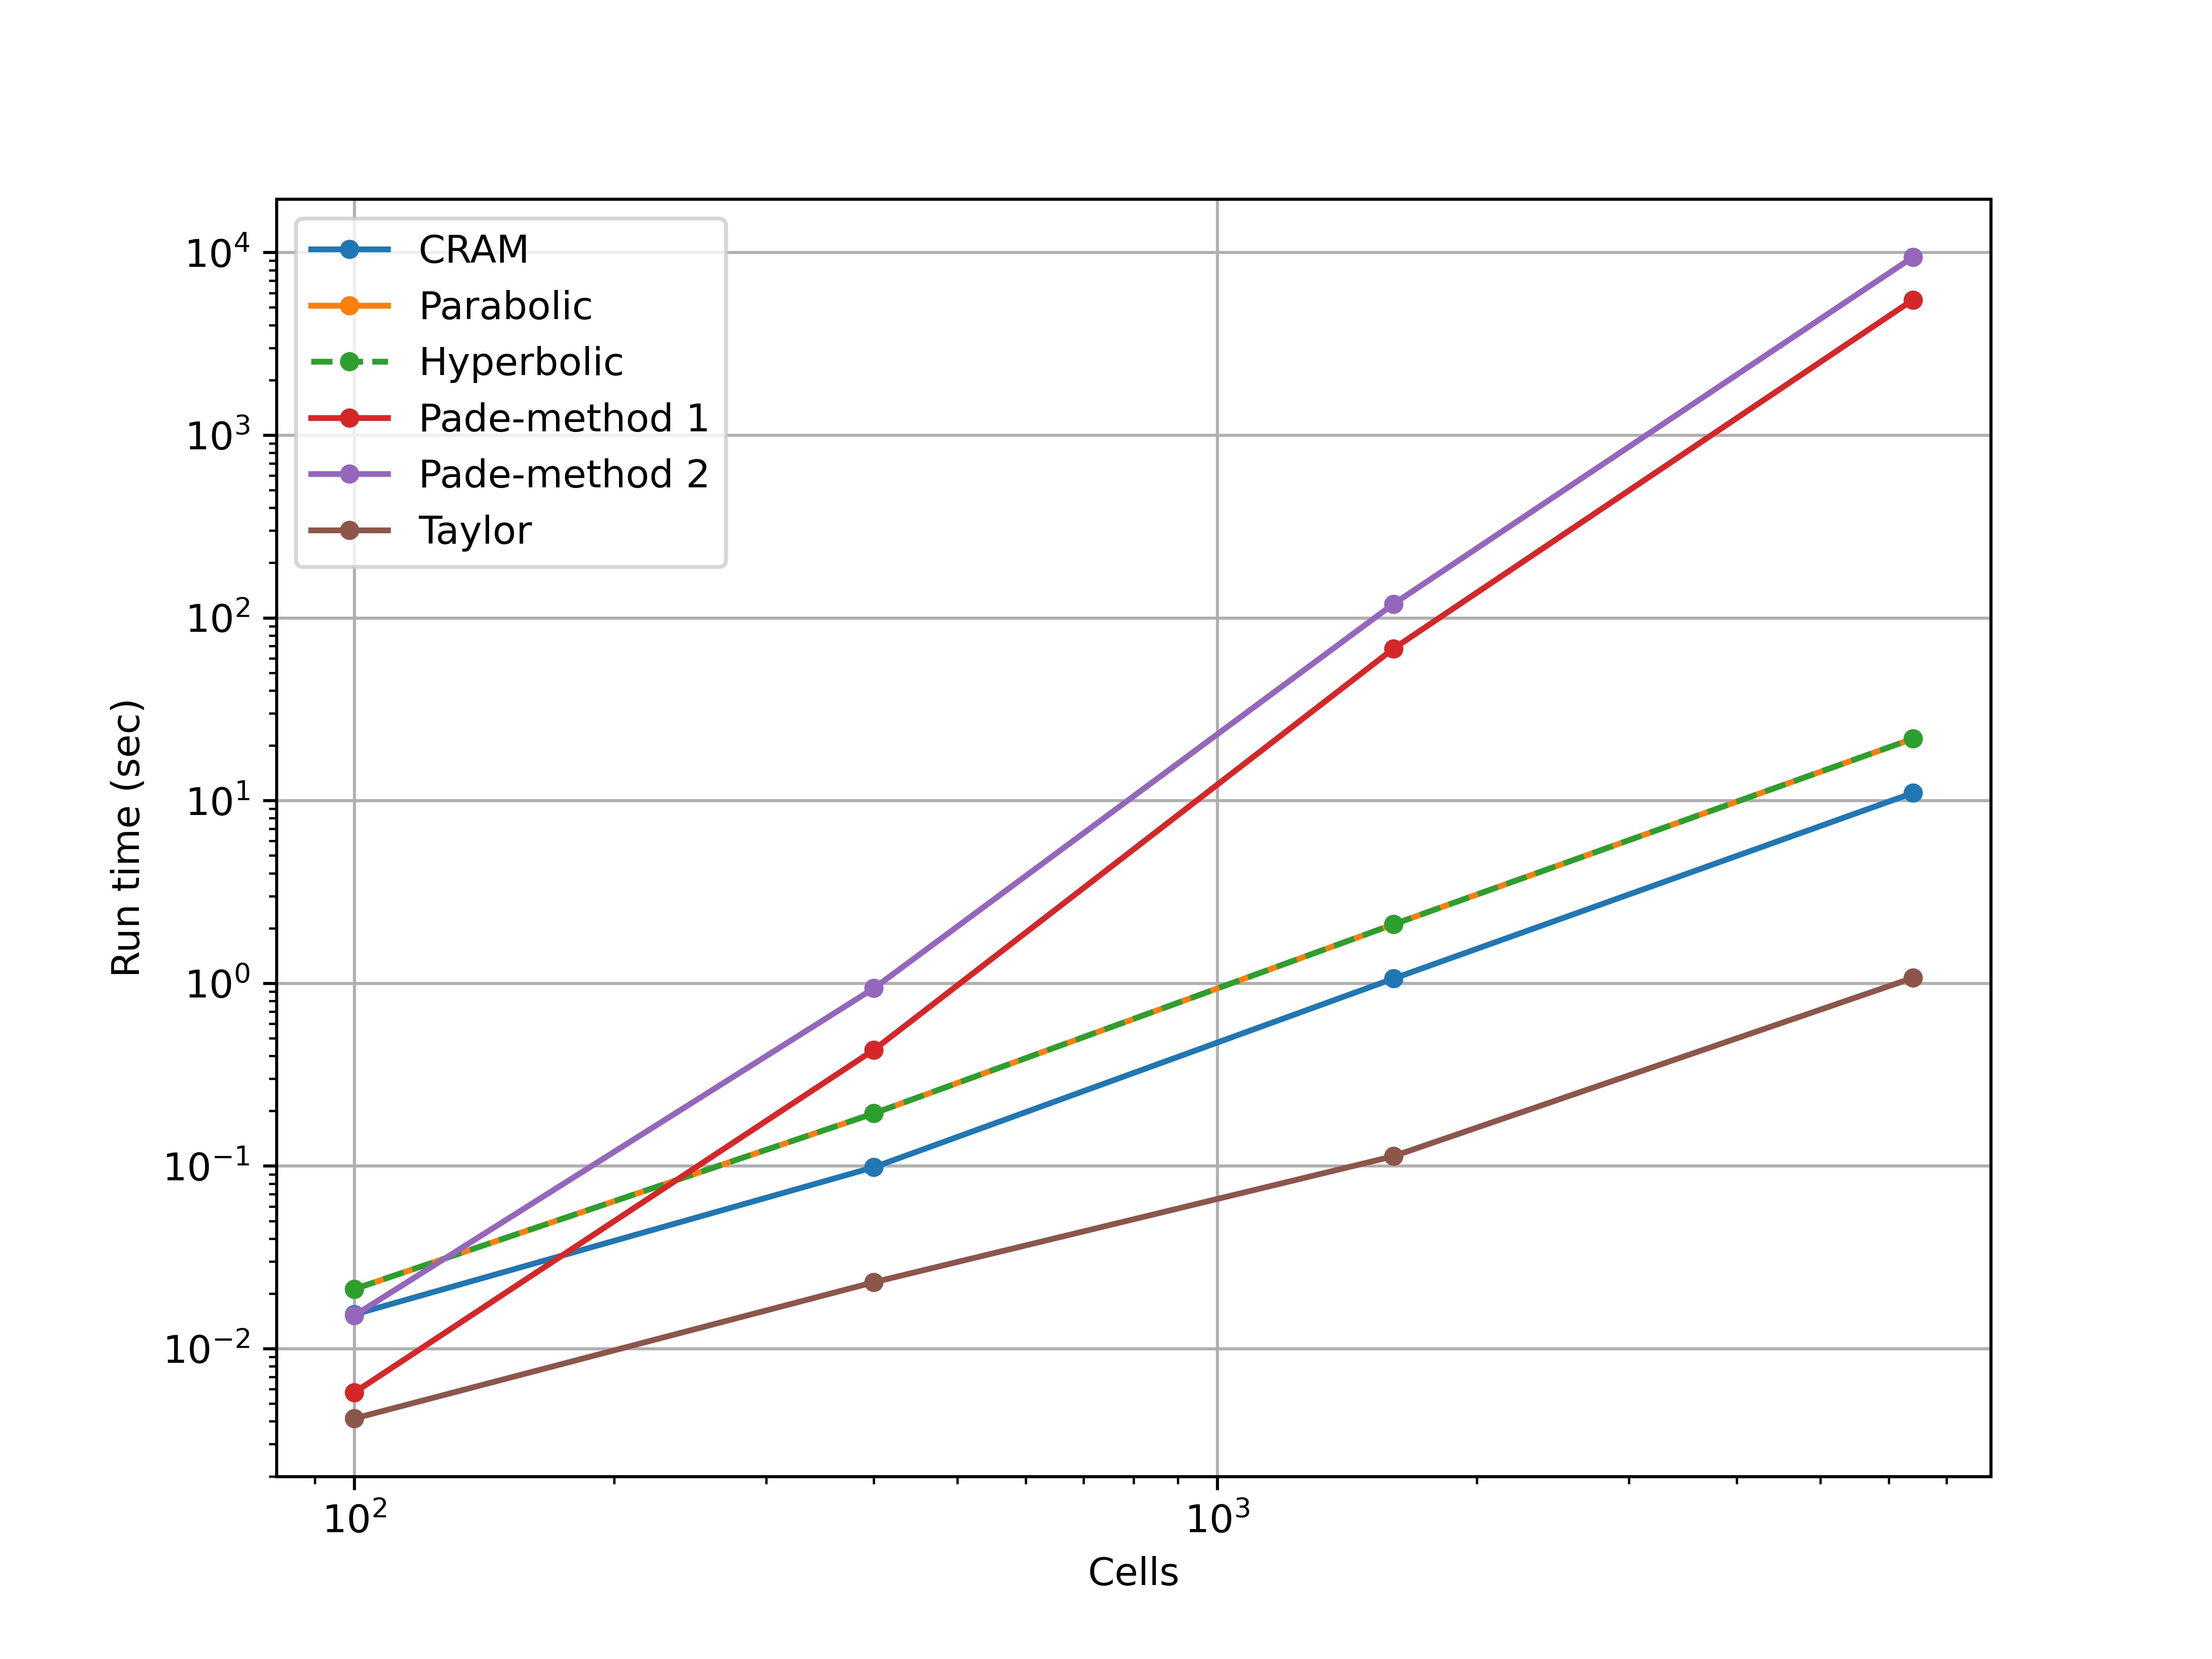
\includegraphics[width=3.9in]{images/chapter-5/progressionProblems/problem1/diffusionProblem1Runtime.png}
    \caption{Run time performance for diffusion problem one}
    \label{fig:runtime_diffusion_one}
\end{figure}

\begin{figure}[hb]
    \centering
    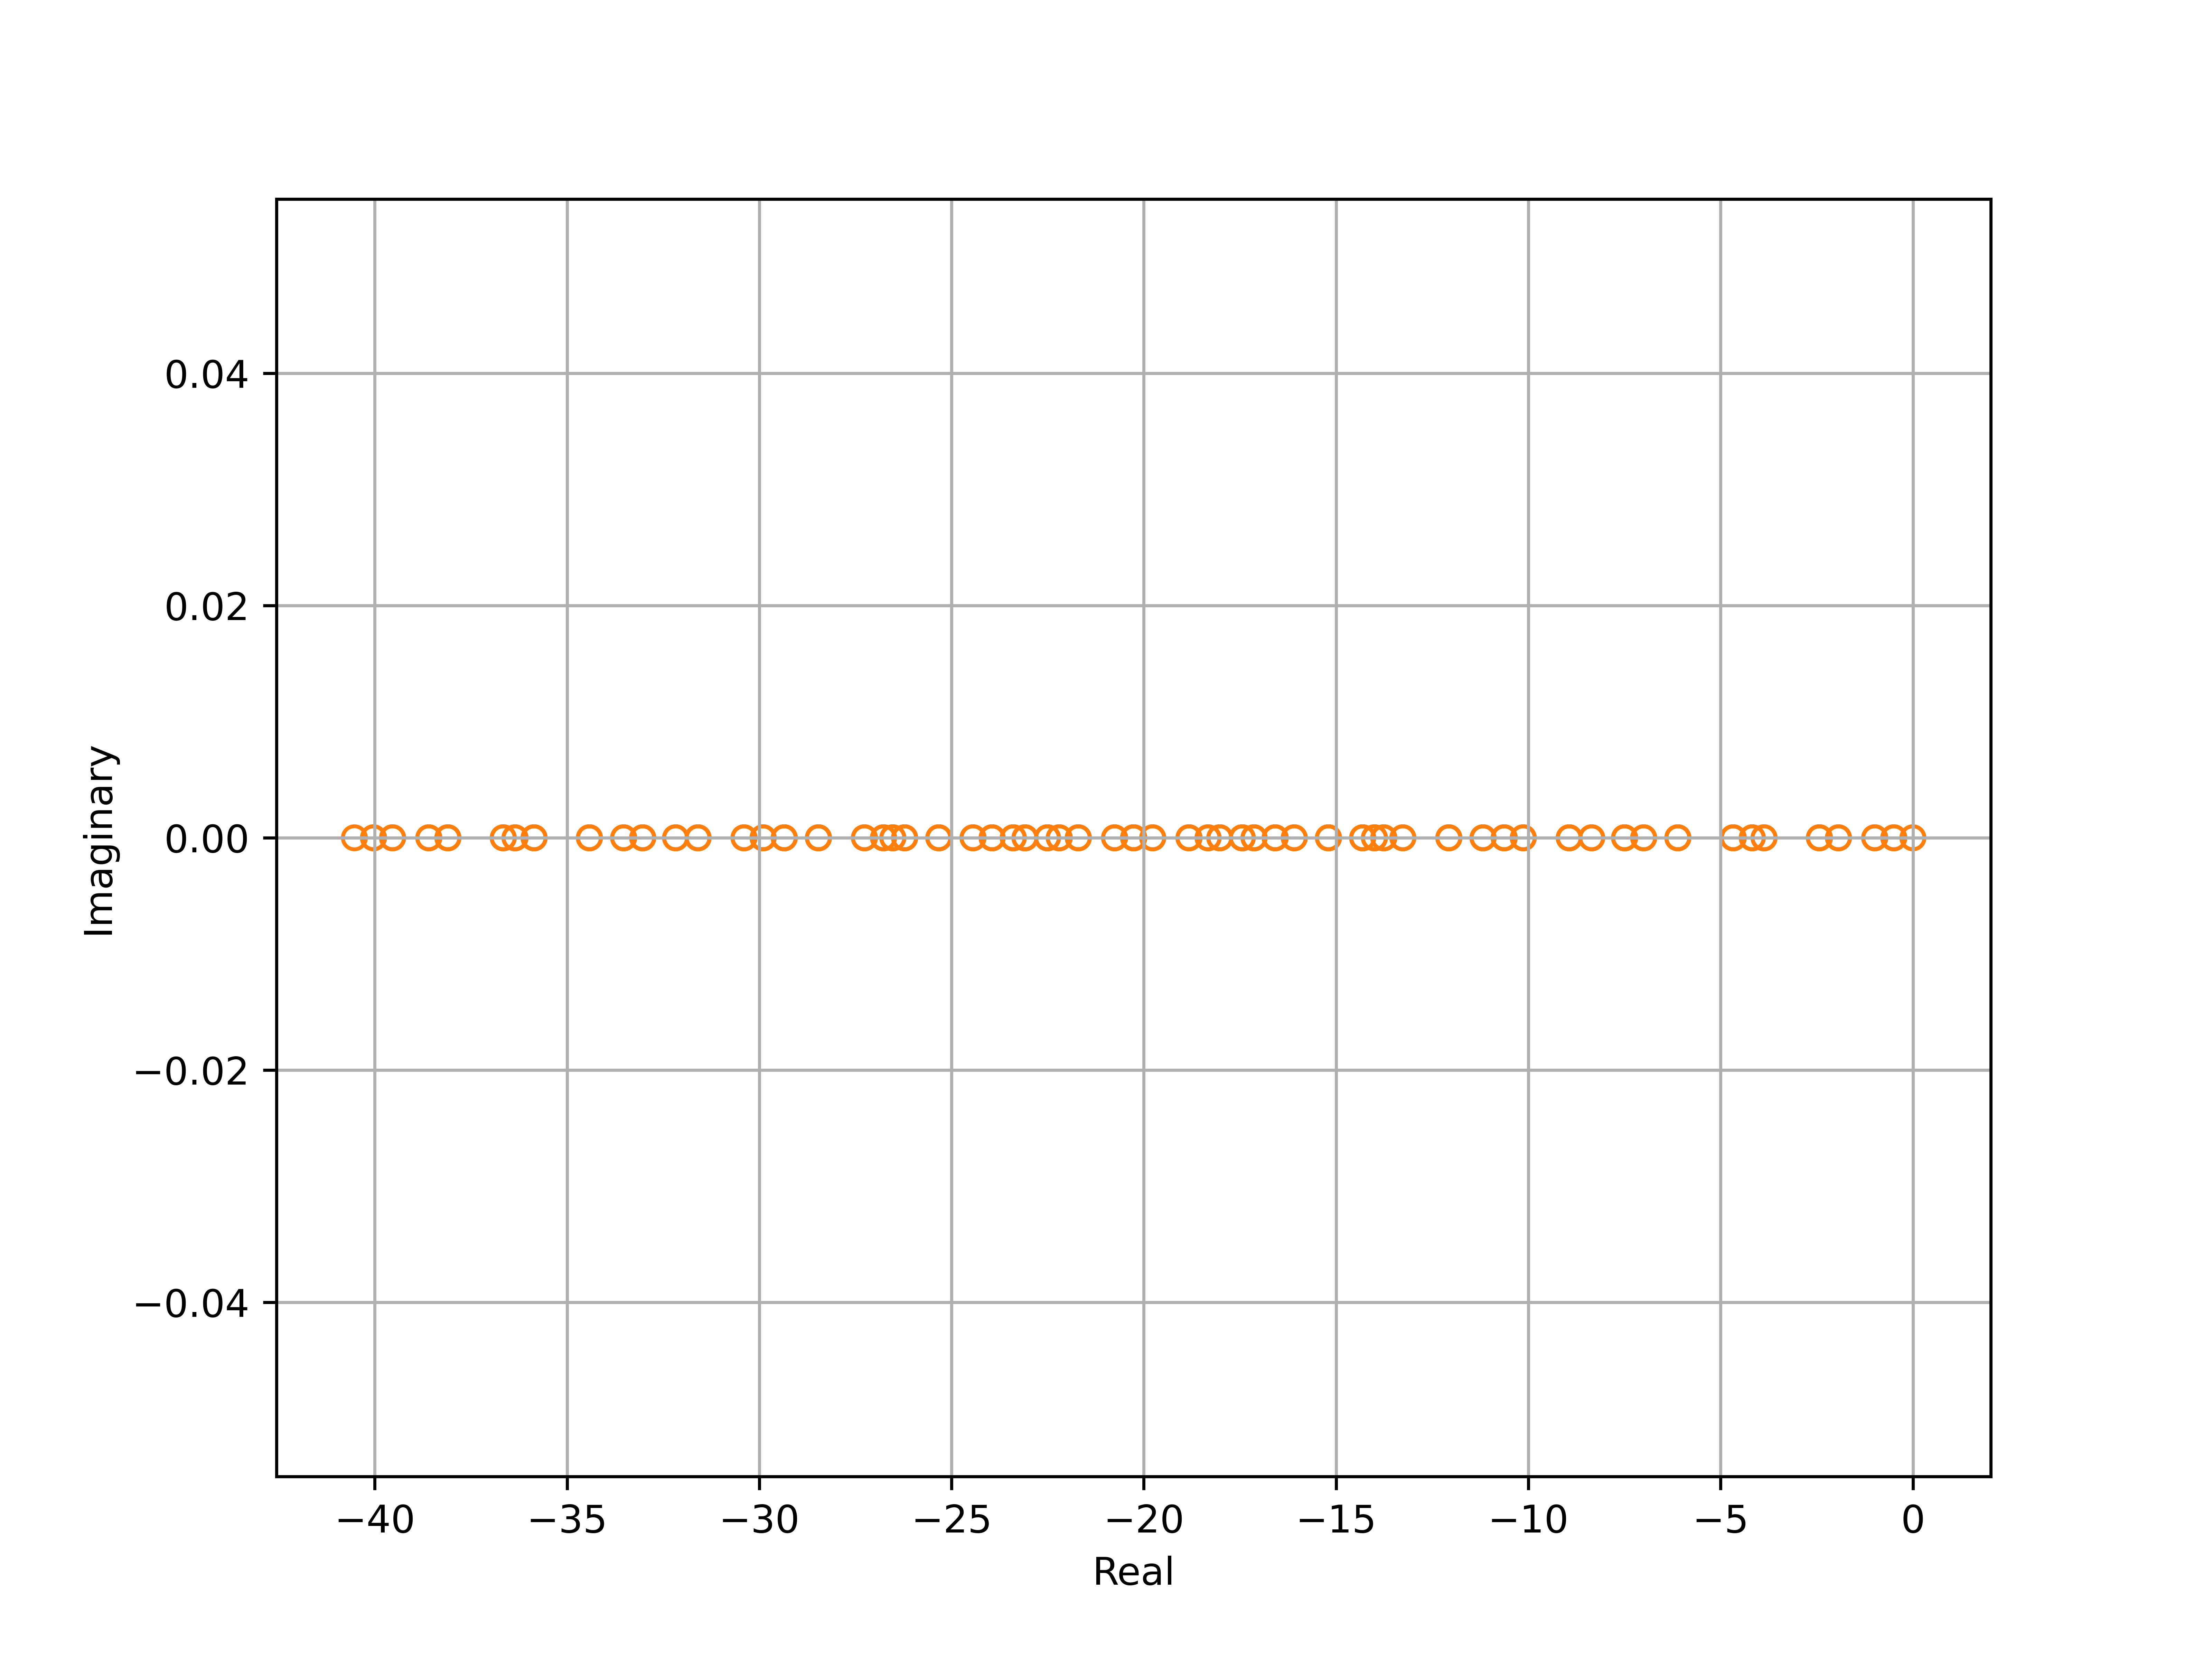
\includegraphics[width=3.9in]{images/chapter-5/progressionProblems/problem1/eigenvaluesDiffusion1-20.png}
    \caption{Eigenvalues for the 400 x 400 case in diffusion problem one}
    \label{fig:eigenvalues_diffusion_one}
\end{figure}

\clearpage

\begin{table}[p]
   \caption{\label{tab:diffusion_problem1_results_krylov} Error and Run Times for Different Krylov Subspace Dimensions}
   \centering
   \begin{tabular}{cllllll}
   \hline
   Solver & M & $l_{\infty}$ Error & $l_{1}$ Error & $l_{2}$ Error & Run time (sec)\\
   \hline
   Pad\'e-method 1 &   5 & 1.74e-05 & 7.05e-06 & 1.12e-02 & 1.13e-02 \\
   - &  10 & 1.74e-05 & 7.05e-06 & 1.12e-02 & 1.47e-02 \\
   - &  25 & 1.74e-05 & 7.05e-06 & 1.12e-02 & 3.31e-02 \\
   - &  50 & 1.74e-05 & 7.05e-06 & 1.12e-02 & 9.27e-02 \\
   - & 100 & 1.74e-05 & 7.05e-06 & 1.12e-02 & 3.33e-01 \\
   - & 150 & 1.74e-05 & 7.05e-06 & 1.12e-02 & 7.30e-01 \\
   - & 200 & 1.74e-05 & 7.05e-06 & 1.12e-02 & 1.33e+00 \\
   \hline
   Pad\'e-method 2 &   5 & 1.74e-05 & 7.05e-06 & 1.12e-02 & 9.15e-03 \\
   - &  10 & 1.74e-05 & 7.05e-06 & 1.12e-02 & 1.18e-02 \\
   - &  25 & 1.74e-05 & 7.05e-06 & 1.12e-02 & 2.96e-02 \\
   - &  50 & 1.74e-05 & 7.05e-06 & 1.12e-02 & 8.95e-02 \\
   - & 100 & 1.74e-05 & 7.05e-06 & 1.12e-02 & 3.28e-01 \\
   - & 150 & 1.74e-05 & 7.05e-06 & 1.12e-02 & 8.20e-01 \\
   - & 200 & 1.74e-05 & 7.05e-06 & 1.12e-02 & 1.55e+00 \\
   \hline
   \end{tabular}
\end{table}


\FloatBarrier
\clearpage

\subsection{Problem 2}
In the second example, a 1D reaction-diffusion problem was modeled. This problem was taken from work performed by Chou et al. (\cite{ching2007}). The partial differential equations (PDEs) are as follows:

\begin{equation}
\setlength{\jot}{15pt}
\begin{split}
    \frac{\partial U}{\partial t} &= d\frac{\partial^{2}U}{\partial x^{2}} - aU + V, \\
    \frac{\partial V}{\partial t} &=
    d\frac{\partial^{2}V}{\partial x^{2}} - bV,
\end{split}
    \label{eq:problem2Eqs}
\end{equation}

\noindent on the domain $x \in [0, \pi/2]$. The system is subject to the following boundary conditions: 

\begin{equation}
    \frac{\partial U}{\partial x}(0,t) = 0, \quad \frac{\partial V}{\partial x}(0,t) = 0, \quad U(\frac{\pi}{2}, t) = 0, \quad V(\frac{\pi}{2}, t)= 0,
\end{equation}

\noindent with the following initial condition:

\begin{equation}
    U(x,0) = 2\cos(x), \quad V(x,0) = (a-b)\cos(x).
\end{equation}

\noindent The exact solution is given by

\begin{equation}
\setlength{\jot}{15pt}
\begin{split}
    U(x,t) = \bigg( e^{-(a+d)t} + e^{-(b+d)t}\bigg)\cos(x), \text{ and} \\
    V(x,t) = (a - b) e^{-(b+d)t}\cos(x).
\end{split}
\end{equation}

The same three test problems that were conducted in the work by Chou et al. (\cite{ching2007}) were also conducted in libowski. These test results correspond to changes in coefficients $[a, b, d]$, which produced a diffusion-dominated system [0.1, 0.01, 1.0], a reaction-dominated system [2.0, 1.0, 0.001], and a stiff reaction system [100, 1.0, 0.001]. Each test case was run with one time step to $t = 1$, so $\Delta t = 1$. The number of cells in the x direction was varied from 10 to 320. Results for the spatial convergence for the Taylor solver for the diffusion-dominated, reaction-dominated and stiff reaction--dominated cases are shown in Tables \ref{tab:diffusion_spatial_convergence_diffusion_dom}, \ref{tab:diffusion_spatial_convergence_reaction_dom}, and \ref{tab:diffusion_spatial_convergence_stiff_reaction_dom}. Each solver produced the same error at up to four decimal places for most of the $n$ values; therefore, only the Taylor results are shown. Full results for these test are shown in Appendix \ref{appen:results} Tables \ref{tab:diffusion_diffusion_dom_problem2_results}, \ref{tab:diffusion_reaction_dom_problem2_results} and \ref{tab:diffusion_stiff_reaction_dom_problem2_results}. As expected, the convergence rate for this problem is second order or better for each of the error metrics.  While there is little difference between the errors from these solvers for this first problem, there is a notable difference in run times for the Pad\'e and Taylor solvers. The E${}_{\infty}$ error and run time for each sub-problem is shown in Figures \ref{fig:problem2_diffusion_dom}, \ref{fig:problem2_reaction_dom} and \ref{fig:problem2_stiff_reaction_dom}. 

Figures \ref{fig:problem2_diffusion_dom}-\ref{fig:problem2_stiff_reaction_dom} show that CRAM is the fastest solver, followed by the parabolic and hyperbolic solvers. Both of the Pad\'e solvers had drastically much longer run times for the diffusion-dominated cases, with Method 2 being the longest. Interestingly, the Taylor solver showed dramatically different run times based on the physical process dominating the problem. In the diffusion-dominated cases, the Taylor solver took the longest, but in the reaction-dominated cases, the run time was on the order of the CRAM, parabolic, and hyperbolic solvers. 

The Krylov subspace approximation was applied to each sub-problem with 1,000 cells in the x direction. The Krylov dimensions were varied from 2 to 100, and the results are shown in Figure \ref{fig:problem2_krylov} . Unlike the previous diffusion example, a much larger Krylov dimension was required to reach a converged error in the diffusion-dominated case. Each solver showed the same error behavior, but with slightly different converged errors due to numerical accuracy in the algorithms. Each solver also showed similar behavior, with run time scaling as a function of the Krylov dimension; however, each axis was scaled differently. Applying the Krylov subspace to each Pad\'e solver reduced the many orders of magnitude, but it failed to reduce the run time of the Taylor solver to the same order in the diffusion-dominated case. For each of the reaction-dominated cases, the Krylov subspace dimension required to reach a converged solution is much smaller than the diffuion-dominated case. 

\clearpage

\begin{table}[h]
   \caption{\label{tab:diffusion_spatial_convergence_diffusion_dom} Convergence Rate for Diffusion-Dominated Problem Using Absolute Error}
   \centering
   \begin{tabular}{lllllll}
   \hline
    n & E${}_{\infty}$ Rate & E${}_{1}$ Rate & E${}_{2}$ Rate & E${}_{\infty}$ Error & E${}_{1}$ Error & E${}_{2}$ Error\\
   \hline
    20 & 2.00 & 2.00 & 2.50 & 1.87e-04 & 1.19e-04 & 2.97e-05 \\ 
    40 & 2.00 & 2.00 & 2.50 & 4.69e-05 & 2.99e-05 & 5.24e-06 \\ 
    80 & 2.00 & 2.00 & 2.50 & 1.17e-05 & 7.46e-06 & 9.27e-07 \\ 
   160 & 2.00 & 2.00 & 2.50 & 2.93e-06 & 1.87e-06 & 1.64e-07 \\ 
   320 & 2.00 & 2.00 & 2.50 & 7.33e-07 & 4.66e-07 & 2.90e-08 \\ 
   \hline
   \end{tabular}
\end{table}

\begin{table}[h]
   \caption{\label{tab:diffusion_spatial_convergence_reaction_dom} Convergence Rate for Reaction-Dominated Problem Using Absolute Error}
   \centering
   \begin{tabular}{lllllll}
   \hline
    n & E${}_{\infty}$ Rate & E${}_{1}$ Rate & E${}_{2}$ Rate & E${}_{\infty}$ Error & E${}_{1}$ Error & E${}_{2}$ Error\\
   \hline
    20 & 2.00 & 2.00 & 2.50 & 2.23e-04 & 1.42e-04 & 3.53e-05 \\  
    40 & 2.00 & 2.00 & 2.50 & 5.58e-05 & 3.55e-05 & 6.24e-06 \\  
    80 & 2.00 & 2.00 & 2.50 & 1.40e-05 & 8.88e-06 & 1.10e-06 \\  
   160 & 2.00 & 2.00 & 2.50 & 3.49e-06 & 2.22e-06 & 1.95e-07 \\  
   320 & 2.00 & 2.00 & 2.50 & 8.72e-07 & 5.55e-07 & 3.45e-08 \\  
   \hline
   \end{tabular}
\end{table}

\begin{table}[h]
   \caption{\label{tab:diffusion_spatial_convergence_stiff_reaction_dom} Convergence Rate for Stiff Reaction--Dominated Problem Using Absolute Error}
   \centering
   \begin{tabular}{lllllll}
   \hline
    n & E${}_{\infty}$ Rate & E${}_{1}$ Rate & E${}_{2}$ Rate & E${}_{\infty}$ Error & E${}_{1}$ Error & E${}_{2}$ Error\\
   \hline
    20 & 2.00 & 2.00 & 2.50 & 9.42e-03 & 6.00e-03 & 1.49e-03 \\ 
    40 & 2.00 & 2.00 & 2.50 & 2.36e-03 & 1.50e-03 & 2.63e-04 \\ 
    80 & 2.00 & 2.00 & 2.50 & 5.89e-04 & 3.75e-04 & 4.66e-05 \\ 
   160 & 2.00 & 2.00 & 2.50 & 1.47e-04 & 9.38e-05 & 8.23e-06 \\ 
   320 & 2.00 & 2.00 & 2.50 & 3.68e-05 & 2.34e-05 & 1.46e-06 \\ 
   \hline
   \end{tabular}
\end{table}

\clearpage

\begin{figure}[p]
    \centering
    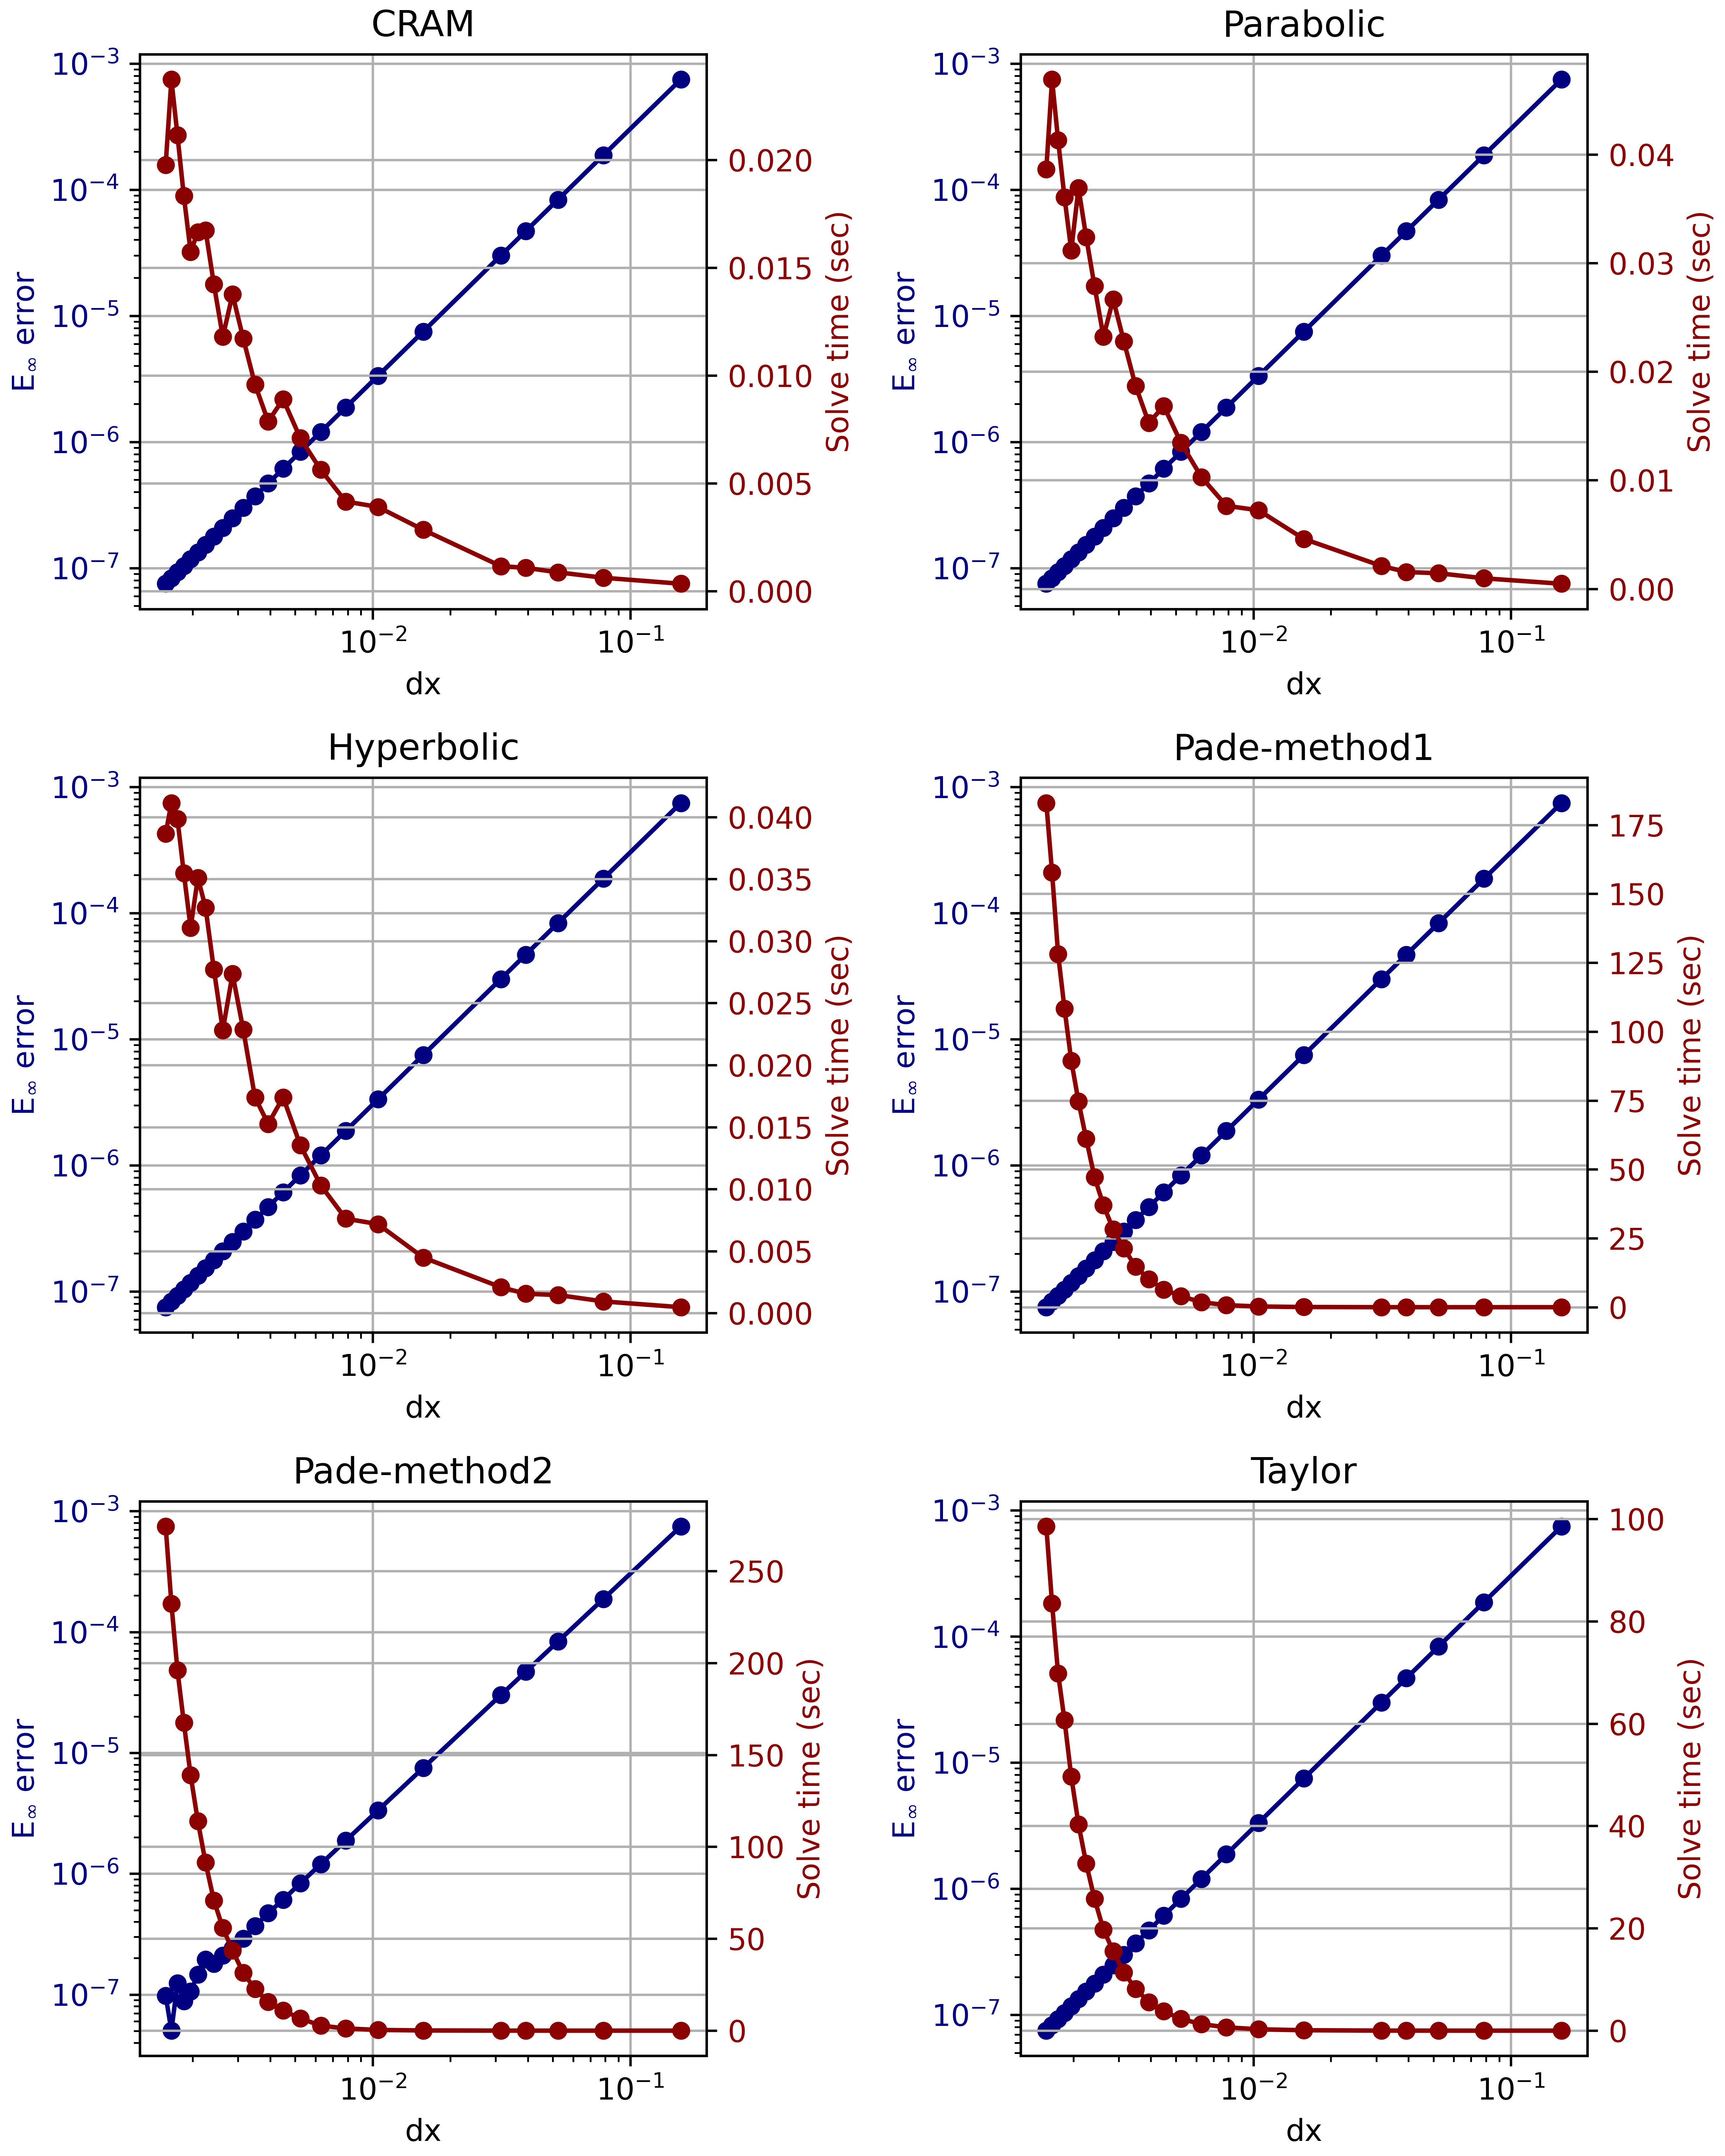
\includegraphics[width=5.0in]{images/chapter-5/progressionProblems/problem2/problem2a.png}
    \caption{Results for the diffusion-dominated case}
    \label{fig:problem2_diffusion_dom}
\end{figure}

\clearpage

\begin{figure}[p]
    \centering
    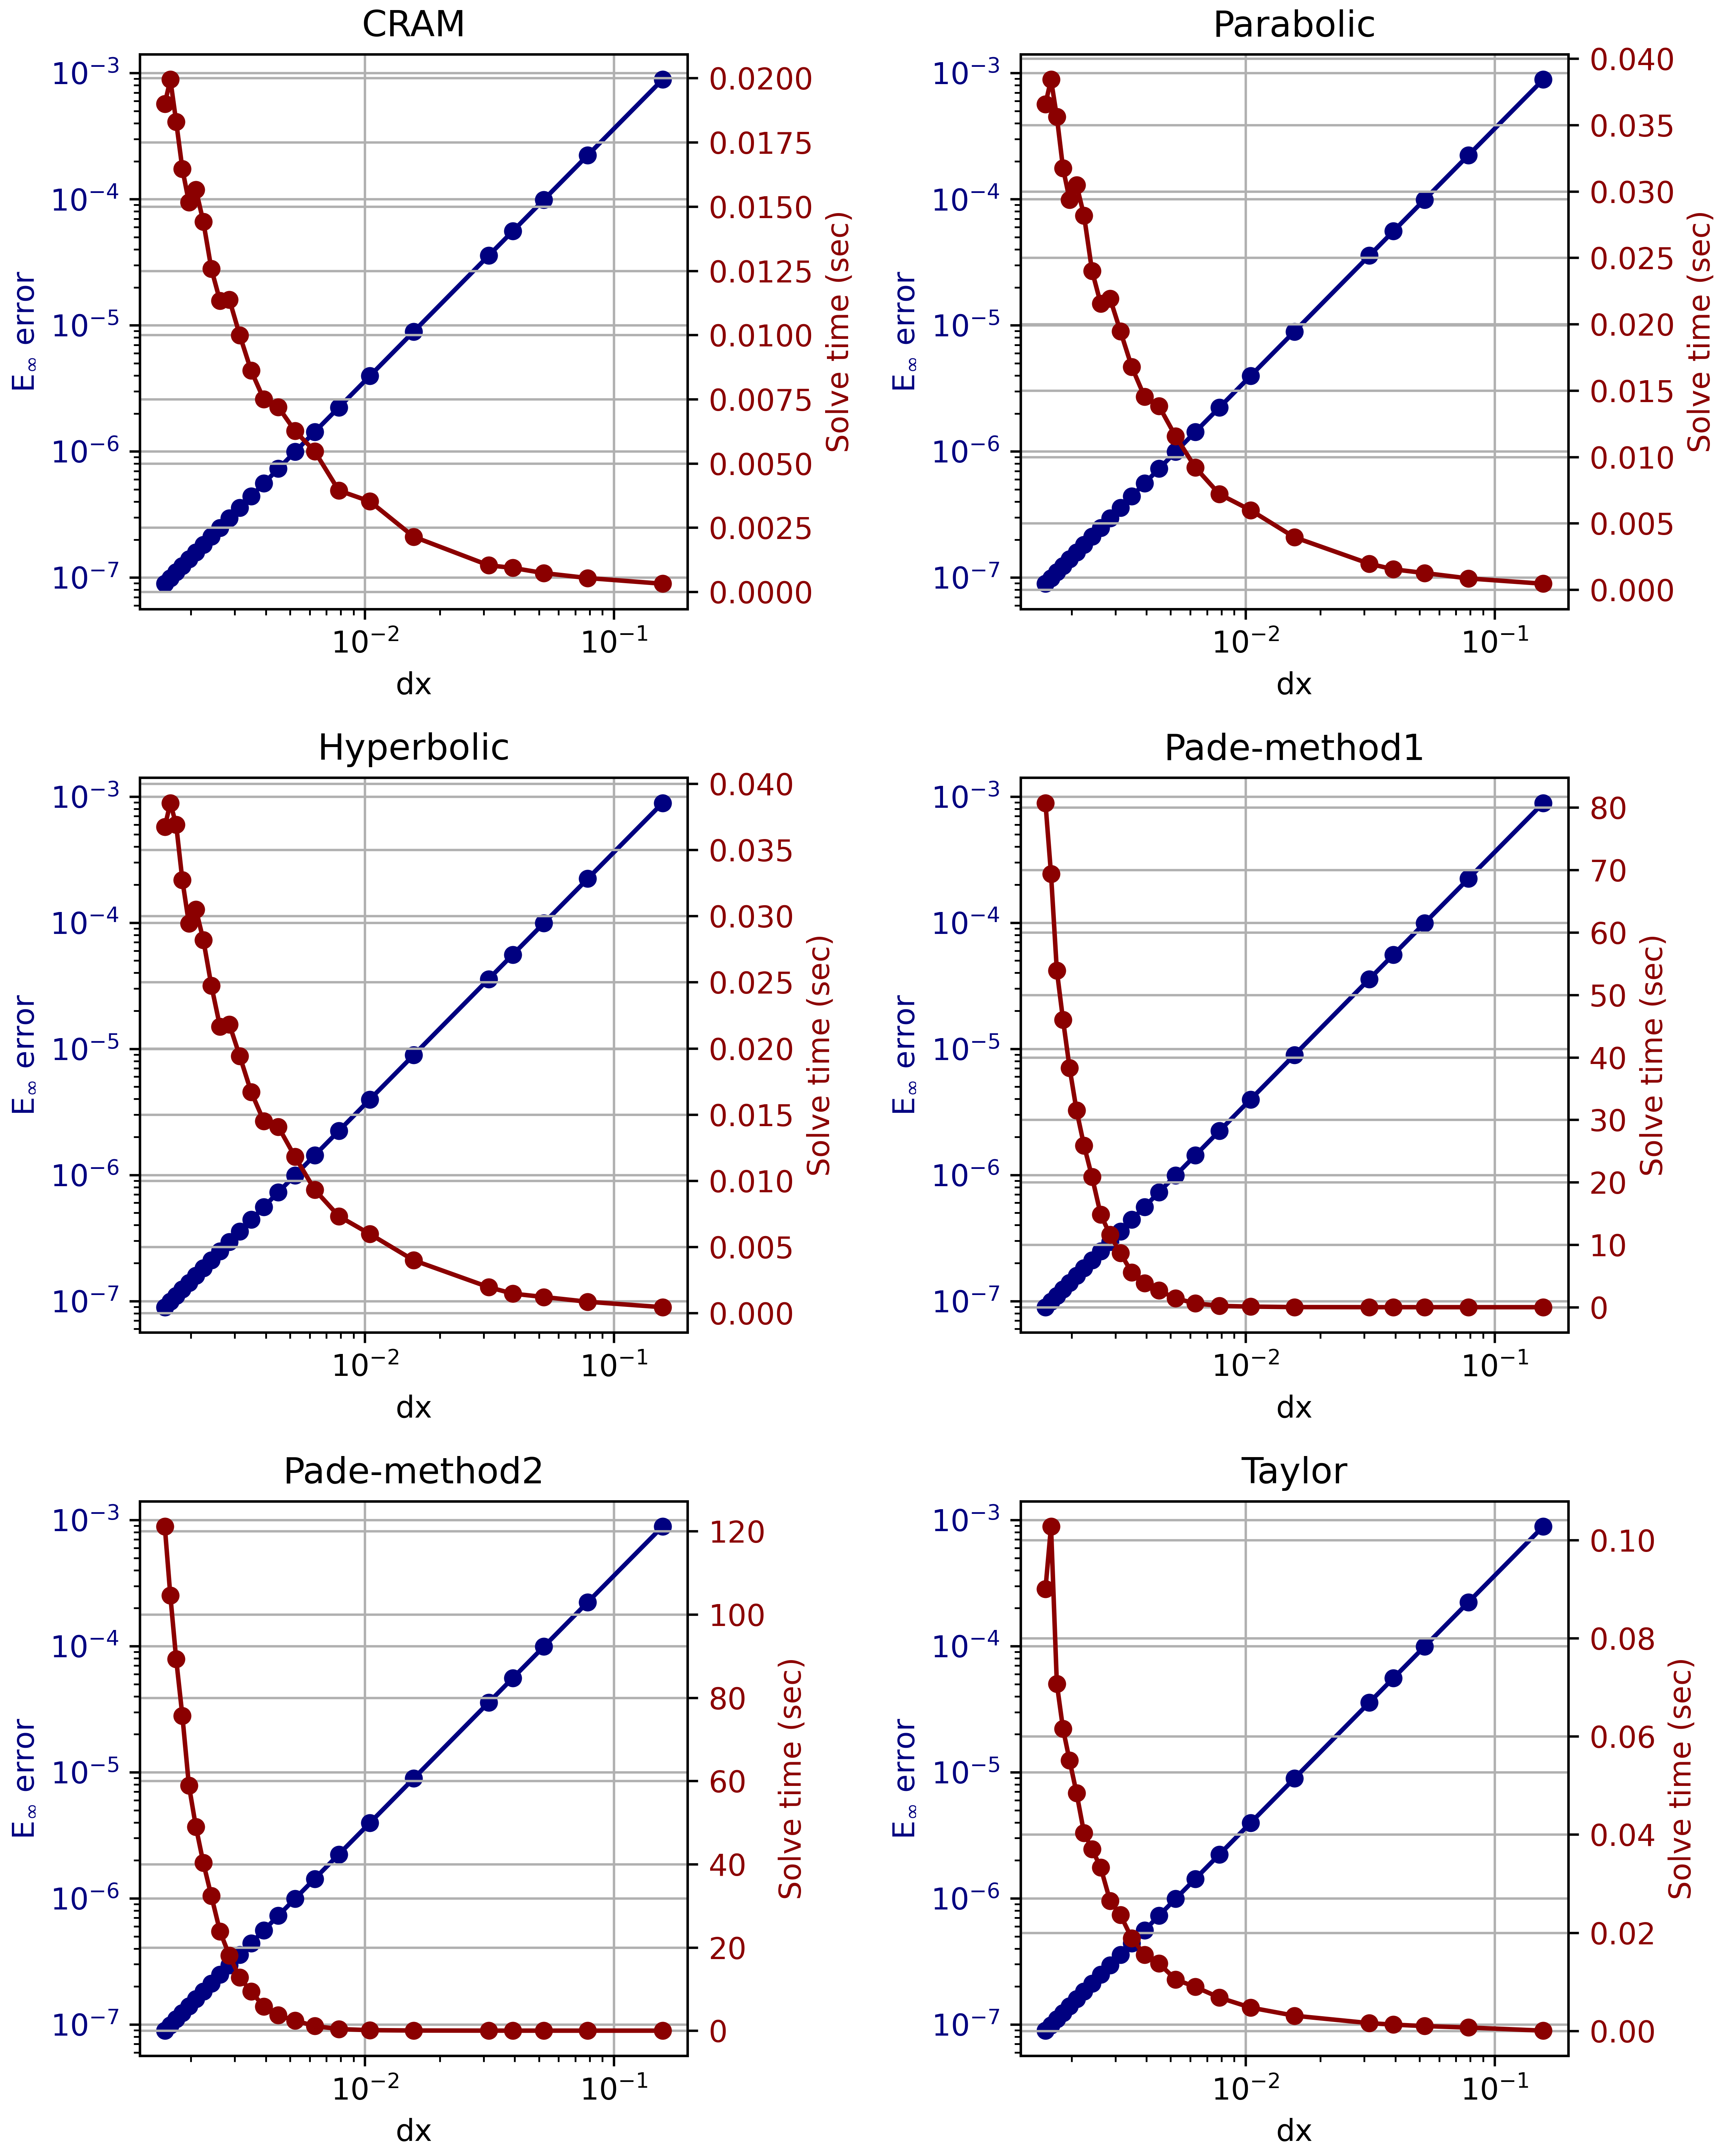
\includegraphics[width=5.0in]{images/chapter-5/progressionProblems/problem2/problem2b.png}
    \caption{Results for the reaction-dominated case}
    \label{fig:problem2_reaction_dom}
\end{figure}

\clearpage

\begin{figure}[p]
    \centering
    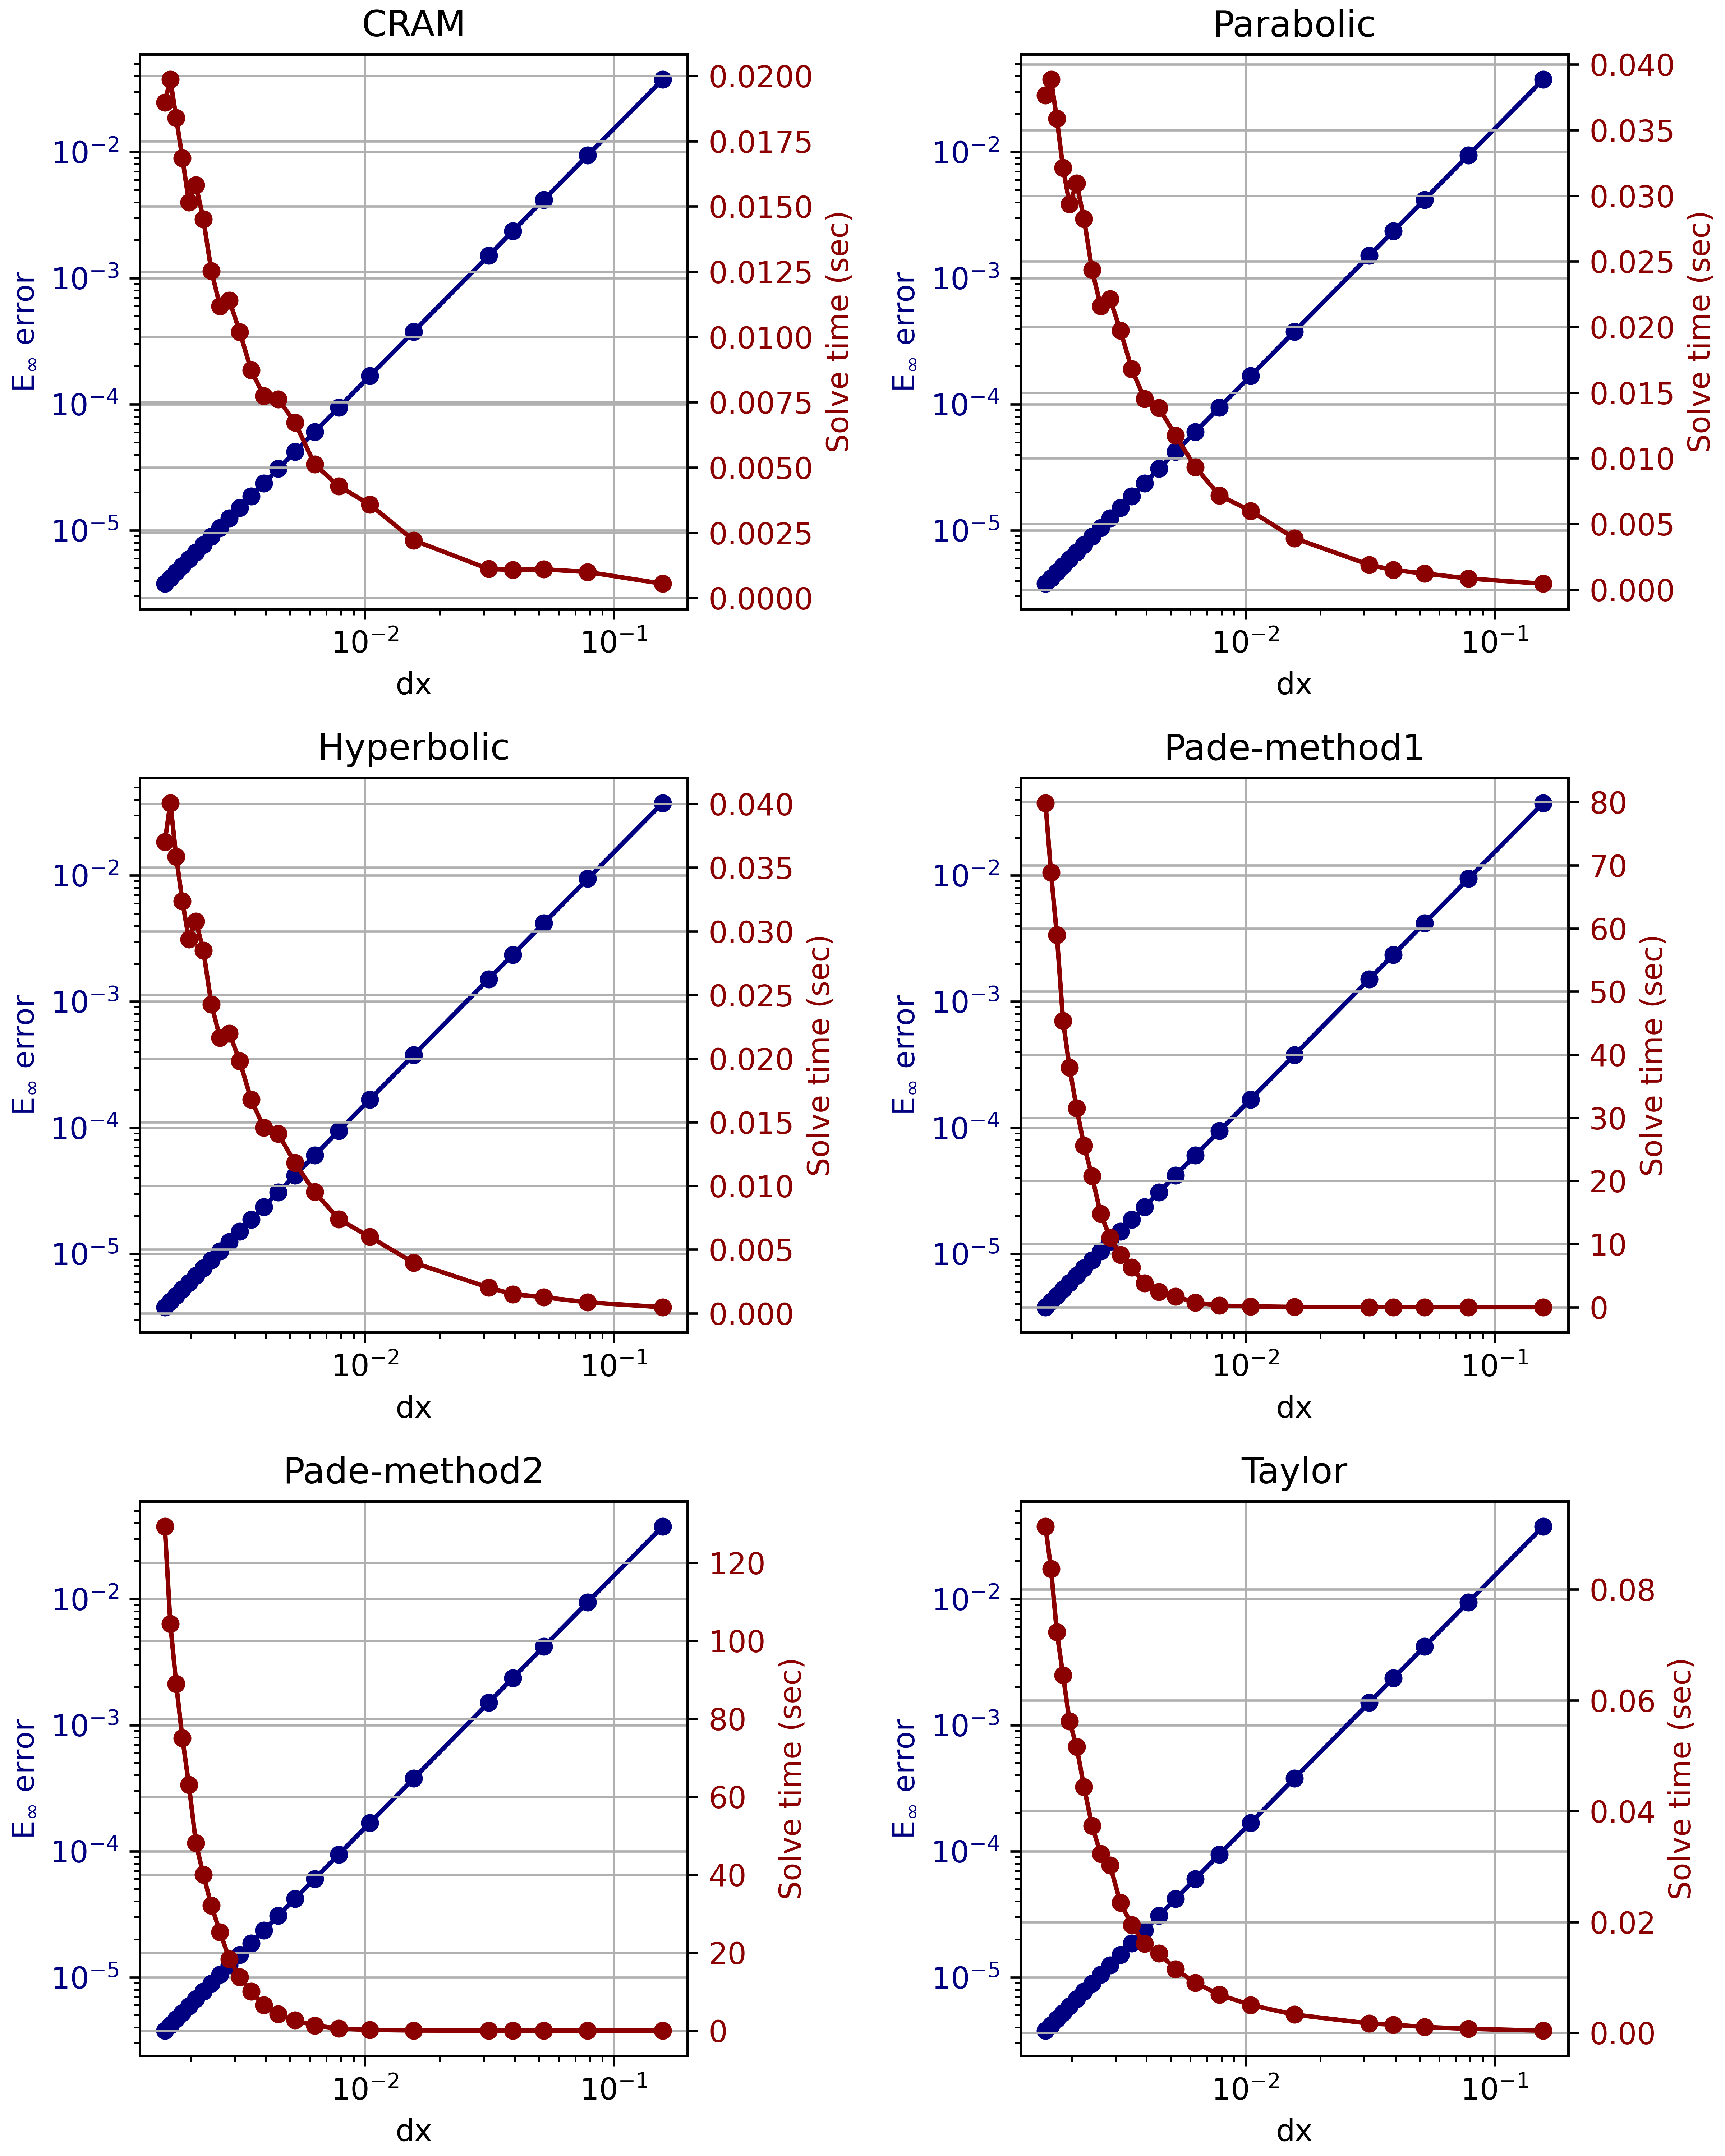
\includegraphics[width=5.0in]{images/chapter-5/progressionProblems/problem2/problem2c.png}
    \caption{Results for the stiff reaction-dominated case}
    \label{fig:problem2_stiff_reaction_dom}
\end{figure}

\clearpage

\begin{sidewaysfigure}[htbp]
    \centering
    \includegraphics[width=8in]{images/chapter-5/progressionProblems/problem2/krylovProblem2.png}
    \caption{Results for the Krylov subspace approximation for each sub-problem}
    \label{fig:problem2_krylov}
\end{sidewaysfigure}

\clearpage

\subsection{Problem 3}

Convection was tested using PDE of the form

\begin{equation}
    \frac{\partial U}{\partial t} = -v\frac{\partial U}{\partial x},
    \label{eq:convection_PDE}
\end{equation}

\noindent where $v$ is velocity. Equation (\ref{eq:convection_PDE}) was applied to a system on the domain $x \in [0, 100]$, $t \in [0, 20]$ subject to the following boundary conditions:

\begin{equation}
    U(0,t) = 1.0, \quad\frac{\partial U}{\partial x}(100, t) = 0.0,
\end{equation}

\noindent and the initial condition:

\begin{equation}
    U(x,0) = 0.0.
\end{equation}

What is most important about this problem is that it exposes an instability with Cauchy solvers which seems to be specific to this problem. This is something that is not seen with the series solvers such as Pad\'e or Taylor. First, results for the first order upwind differencing scheme are shown in Figure \ref{fig:first_order_results}  for a first-order backward differencing formula (BDF1) and the ETD scheme using the series matrix exponential solvers. While only the Taylor solver is shown, results for the Pad\'e solvers are the same. Figure \ref{fig:first_order_results} shows the typical reduction in numerical diffusion with decreasing dx. In figure \ref{fig:first_order_results} we see that as the time step size decreases for the explicit BDF1 solver it approaches the accuracy of the ETD method with a single time step. 

The instability seen with Cauchy solvers is shown in figure \ref{fig:first_order_results_cauchy_instability} for a zoomed in and zoomed out view of each solution. In figure \ref{fig:first_order_results_cauchy_instability} it is seen that for dx values 0.5 and 0.4, the solution blows up and oscillates. What is important to note that even know the solution for dx = 1.0 is stable it does contain small negative values as it approaches zero. The matrix exponential is the analytical solution to the ODE system and should not show any instability, so the instability shown here is due to the numerical computation of the exponential itself. To combat this instability the order of the method can be increased, this is seen in figure \ref{fig:first_order_results_cauchy_instability_different_orders}. Figure \ref{fig:first_order_results_cauchy_instability_different_orders} shows the Hyperbolic and Parabolic solvers at different order of N. As the order in increased, the solution becomes more stable.  Another method to increase the stability of the solution is to compute the solution with multiple steps and not just at the final time step. This is equivalent to using the substep method for the Cauchy solvers. Figure \ref{fig:first_order_results_cauchy_instability_different_time_steps} shows results for each of the Cauchy solver for different time step sizes. Even with large time step sizes the solution becomes stable.   \textcolor{red}{Discuss accuracy related to the Jordan canonical form.}

To illustrate the enhanced accuracy of TVD non-linear flux limiters, the same problem is conducted with a variety of limiter functions. This method works to approximate the convection term to at most second order in the case of smooth solutions and reduce numerical diffusion seen in the first order case. Figure \ref{fig:fluxlimiters_problem3} shows results from each of the flux limiter functions in libowski using the Taylor solver. Each of the flux limiter functions reduces the numerical diffusion, seen in the first order upwind case with superbee being the best. While the TVD scheme is designed to remove unphysical oscillations seen in higher order convection schemes, these oscillations are present because of the explicit implementation. Figure \ref{fig:fluxlimiters_instability_problem3} shows these oscillations for six flux limiter functions. This behavior is only present when large time step sizes are used. For some time integration methods, explicit schemes are known to be unstable if large time step sizes are used. In this case the second order correction being calculated from the previous time step causes the solution to become unstable if large enough time steps are taken. This same behavior is seen in all the ETD matrix exponential solvers. 

\clearpage

\begin{figure}[p]
    \centering
    \includegraphics[width=6in]{images/chapter-5/progressionProblems/problem3/problem3FirstOrder.png}
    \caption{First-order upwind differencing with series solvers and BDF1}
    \label{fig:first_order_results}
\end{figure}

\clearpage

\begin{figure}[p]
    \centering
    \includegraphics[width=6.0in]{images/chapter-5/progressionProblems/problem3/problem3FirstOrderCauchyInstability.png}
    \caption{First-order upwind differencing instability for Cauchy solvers}
    \label{fig:first_order_results_cauchy_instability}
\end{figure}

\clearpage

\begin{figure}[p]
    \centering
    \includegraphics[width=5.0in]{images/chapter-5/progressionProblems/problem3/problem3FirstOrderCauchyInstabilityDifferentOrders.png}
    \caption{First-order upwind differencing instability for Cauchy solvers at different orders}
    \label{fig:first_order_results_cauchy_instability_different_orders}
\end{figure}

\clearpage

\begin{figure}[p]
    \centering
    \includegraphics[width=6in]{images/chapter-5/progressionProblems/problem3/problem3FirstOrderCauchyInstabilityDifferentTimeSteps.png}
    \caption{First-order upwind differencing instability for Cauchy solvers at different time step sizes}
    \label{fig:first_order_results_cauchy_instability_different_time_steps}
\end{figure}

\clearpage

\begin{figure}[p]
    \centering
    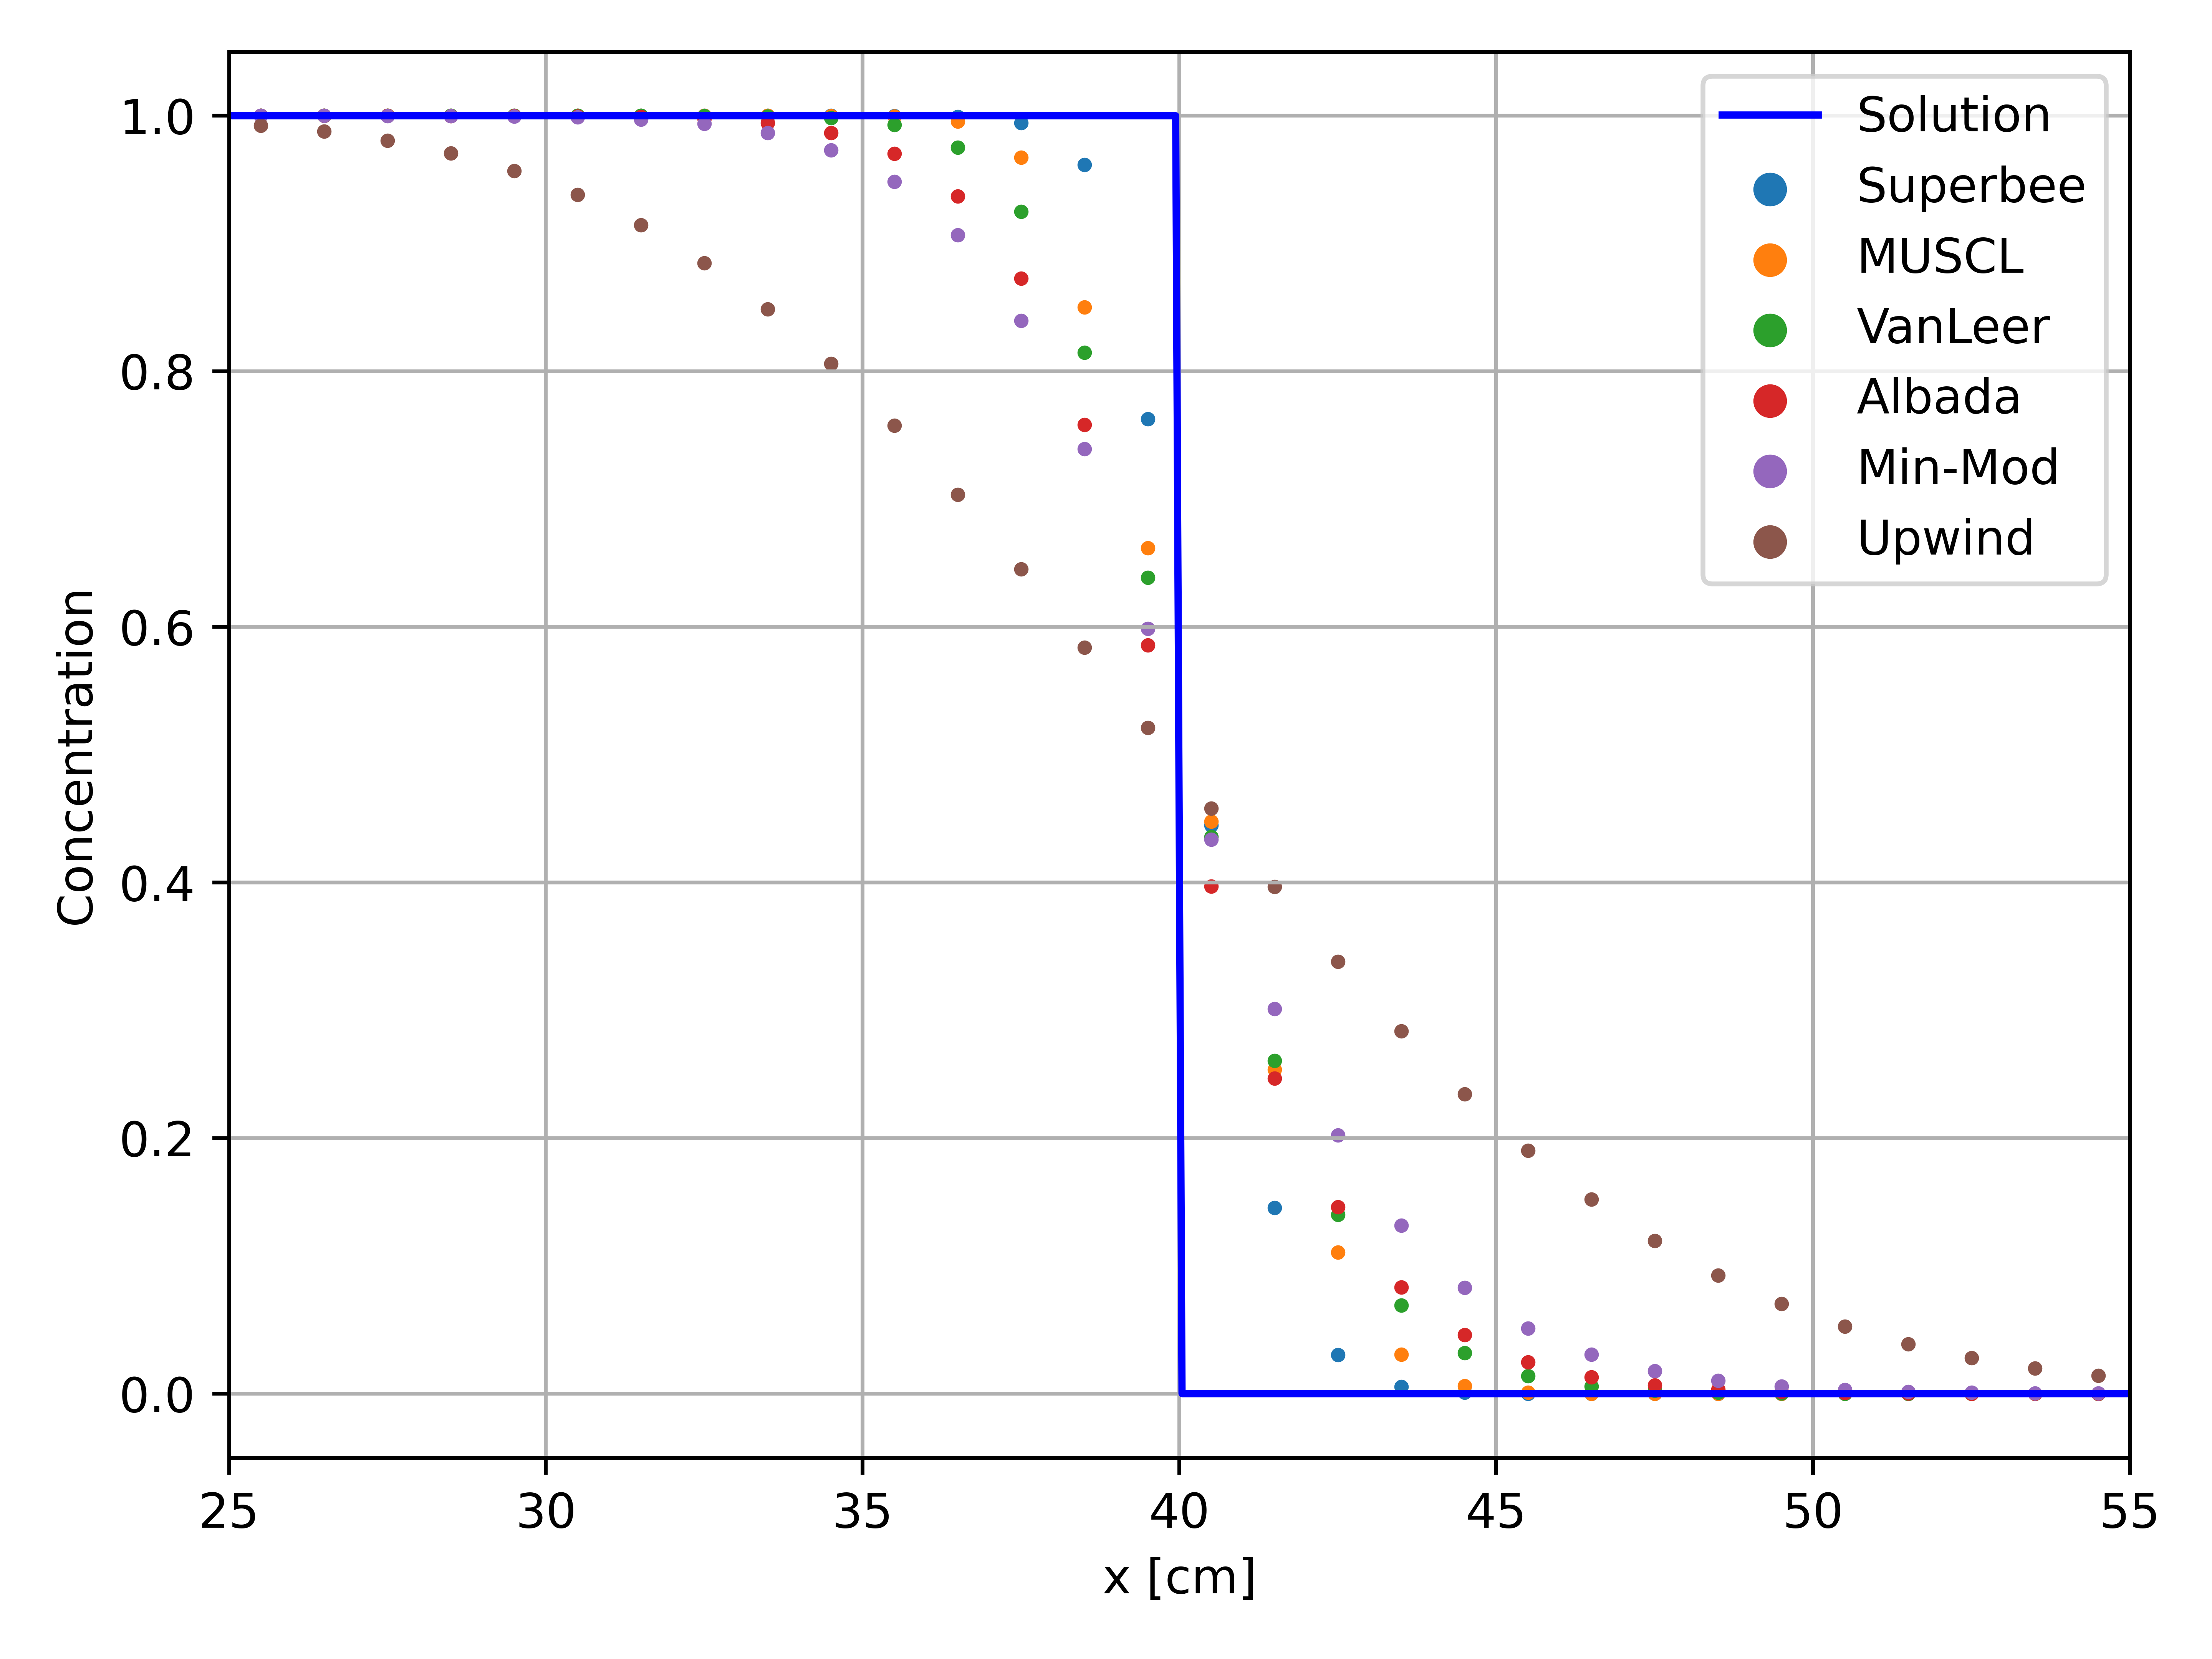
\includegraphics[width=5in]{images/chapter-5/progressionProblems/problem3/problem3FluxLimiters.png}
    \caption{Flux limiter function applied to problem three, dt = 0.1, dx = 0.2}
    \label{fig:fluxlimiters_problem3}
\end{figure}

\clearpage

\begin{figure}[p]
    \centering
    \includegraphics[width=6in]{images/chapter-5/progressionProblems/problem3/problem3SecondOrderFluxLimiterFunctionInstability.png}
    \caption{Instability of flux limiter functions with the Taylor solver}
    \label{fig:fluxlimiters_instability_problem3}
\end{figure}

\clearpage

\subsection{Problem 4}

The same PDE that was shown in the previous problem is tested again:

\begin{equation}
    \frac{\partial U}{\partial t} = -v\frac{\partial U}{\partial x},
    \label{eq:convection_PDE}
\end{equation}

\noindent on the domain $x \in [0, 100]$, $t \in [0, 5]$ subject to periodic boundary conditions:

\begin{equation}
    U(0,t) = U(100, t),
\end{equation}

\noindent and the initial condition:

\begin{equation}
    U(x,0) = \exp\bigg\{-\bigg(\frac{(x-30)}{10}\bigg)^{2}\bigg\}.
\end{equation}

\noindent with the following solution:

\begin{equation}
	U(x,t)_ = \exp\bigg\{-\bigg(\frac{(x-vt-30)}{10}\bigg)^{2}\bigg\}.
\end{equation}

Figure \ref{fig:problem4_l1error_spatial_results} shows E${}_{1}$ error behavior as a function of spatial discretization at various time step sizes. Figure \ref{fig:problem4_l1error_time_results} shows the same error behavior as a function of temporal discretization at various number of spatial cells. Figure \ref{fig:problem4_l1error_spatial_results} shows that as the number of time steps take is increased the higher order flux limiters begin to show a linear relationship with spatial discretization. This can be readily seen with the number of steps greater than 40. The upwind limiter is unaffected by decreasing the time step size, which is to be expected. This is because increasing the number of times steps do nothing to increase its accuracy. Figure \ref{fig:problem4_l1error_time_results} shows that increasing the number of time steps has little to no affect on the error for large spatial discretization. As the number of cells increases, decreasing the time step size has a greater affect on reducing the error. This figure also reiterates the fact that the first order upwind error is not affected by increasing the number of time steps taken. Results for the E${}_{\infty}$ and E${}_{2}$ errors are shown in Appendix \ref{appen:results} figures \ref{fig:problem4_linferror_spatial_results}, \ref{fig:problem4_linferror_time_results}, \ref{fig:problem4_l2error_spatial_results} and \ref{fig:problem4_l2error_time_results}. Figure \ref{fig:problem4_linferror_spatial_results} shows a similar trend with spatial refinement using the E${}_{\infty}$ error to the E${}_{1}$ error however, the error function in figure \ref{fig:problem4_linferror_spatial_results} does not maintain the same linear rate. This relation is further represented in Figure \ref{fig:problem4_linferror_time_results} which shows the error with temporal refinement. For large spatial refinement, the error remains constant. For smaller refinement, the error takes a dip then increases. The E${}_{2}$ error shown in figures \ref{fig:problem4_l2error_spatial_results} and \ref{fig:problem4_l2error_time_results} shows a trend resembling the E${}_{1}$ error, in which the error convergence rate remains semi linear as a function of spatial discretization for most flux limiters with larger number of time steps. 

Figure \ref{fig:problem4_l1error_fluxlimiter_convergence_rate} shows convergence rates for each of the higher order flux limiter functions as a function of space and time using the E${}_{1}$ error. Each flux limiter shows a dark zone (representing low convergence rate) with high spatial discretization and low temporal discretization. At 320 spatial cells, the convergence rate of each flux limiter increases until reaching an apex at 40 time steps, then slightly decreases to a constant-ish value. At low spatial resolution, increases the number of time steps taken does not have a large affect on changing the convergence rate. Results for the E${}_{\infty}$ and E${}_{2}$ error metrics are shown in Appendix \ref{appen:results} figures \ref{fig:problem4_linferror_fluxlimiter_convergence_rate} and \ref{fig:problem4_l2error_fluxlimiter_convergence_rate}. Behavior of the E${}_{2}$ error shows similar trends to $l_{1}$, low convergence rates for high spatial resolution and low temporal, with most limiters showing peak convergence with 8 or 40 time steps and 320 cells. Convergence rates for E${}_{\infty}$ error are shown in figure \ref{fig:problem4_linferror_fluxlimiter_convergence_rate}. These results show convergence rates which are slightly worse than the other two errors. The peak convergence rate for most flux limiters has also shifted from 320 cells and 40 time steps to 320 cells and 8 time steps. All limiter functions also show a general trend of having larger convergence rates at lower spatial resolution. 

Figure \ref{fig:problem4_runtimes} shows the average run time results for each of the solvers. Each flux limiter function call requires the same time meaning that small run time differences for each solve is due to the computers computation. For the small cases, the Taylor and Pad\'e solvers out perform the Cauchy solvers. As the number of cells increase, the Pad\'e solver run times begin to approach values greater than the Cauchy solvers. Hyperbolic and Parabolic remain about the same as seen before, with CRAM being the lowest of the three. The Taylor solver remains the lowest for all problem sizes. 

Unlike the previous example, no instabilities were noticed while conducting the numerical test. Even at large spatial resolutions and small time steps, the flux limiter functions remained stable. Each of the Cauchy solvers also remained stable during testing. While only results for the Taylor solver are shown, all other solvers show the same errors and convergence rates.

\clearpage

\begin{figure}[p]
    \centering
    \includegraphics[width=6in]{images/chapter-5/progressionProblems/problem4/problem4E1ErrorWithSpace.png}
    \caption{Problem 4 absolute E${}_{1}$ error with spatial discretization at various time steps }
    \label{fig:problem4_l1error_spatial_results}
\end{figure}

\clearpage

\begin{figure}[p]
    \centering
    \includegraphics[width=6in]{images/chapter-5/progressionProblems/problem4/problem4E1ErrorWithTime.png}
    \caption{Problem 4 absolute E${}_{1}$ error with temporal discretization at various number of spatial cells}
    \label{fig:problem4_l1error_time_results}
\end{figure}

\clearpage

\begin{figure}[p]
    \centering
    \includegraphics[width=6in]{images/chapter-5/progressionProblems/problem4/problem4E1FluxLimiterConvergenceRate.png}
    \caption{Problem 4 flux limiter E${}_{1}$ spatial convergence rate using absolute error}
    \label{fig:problem4_l1error_fluxlimiter_convergence_rate}
\end{figure}

\clearpage

\begin{figure}[p]
    \centering
    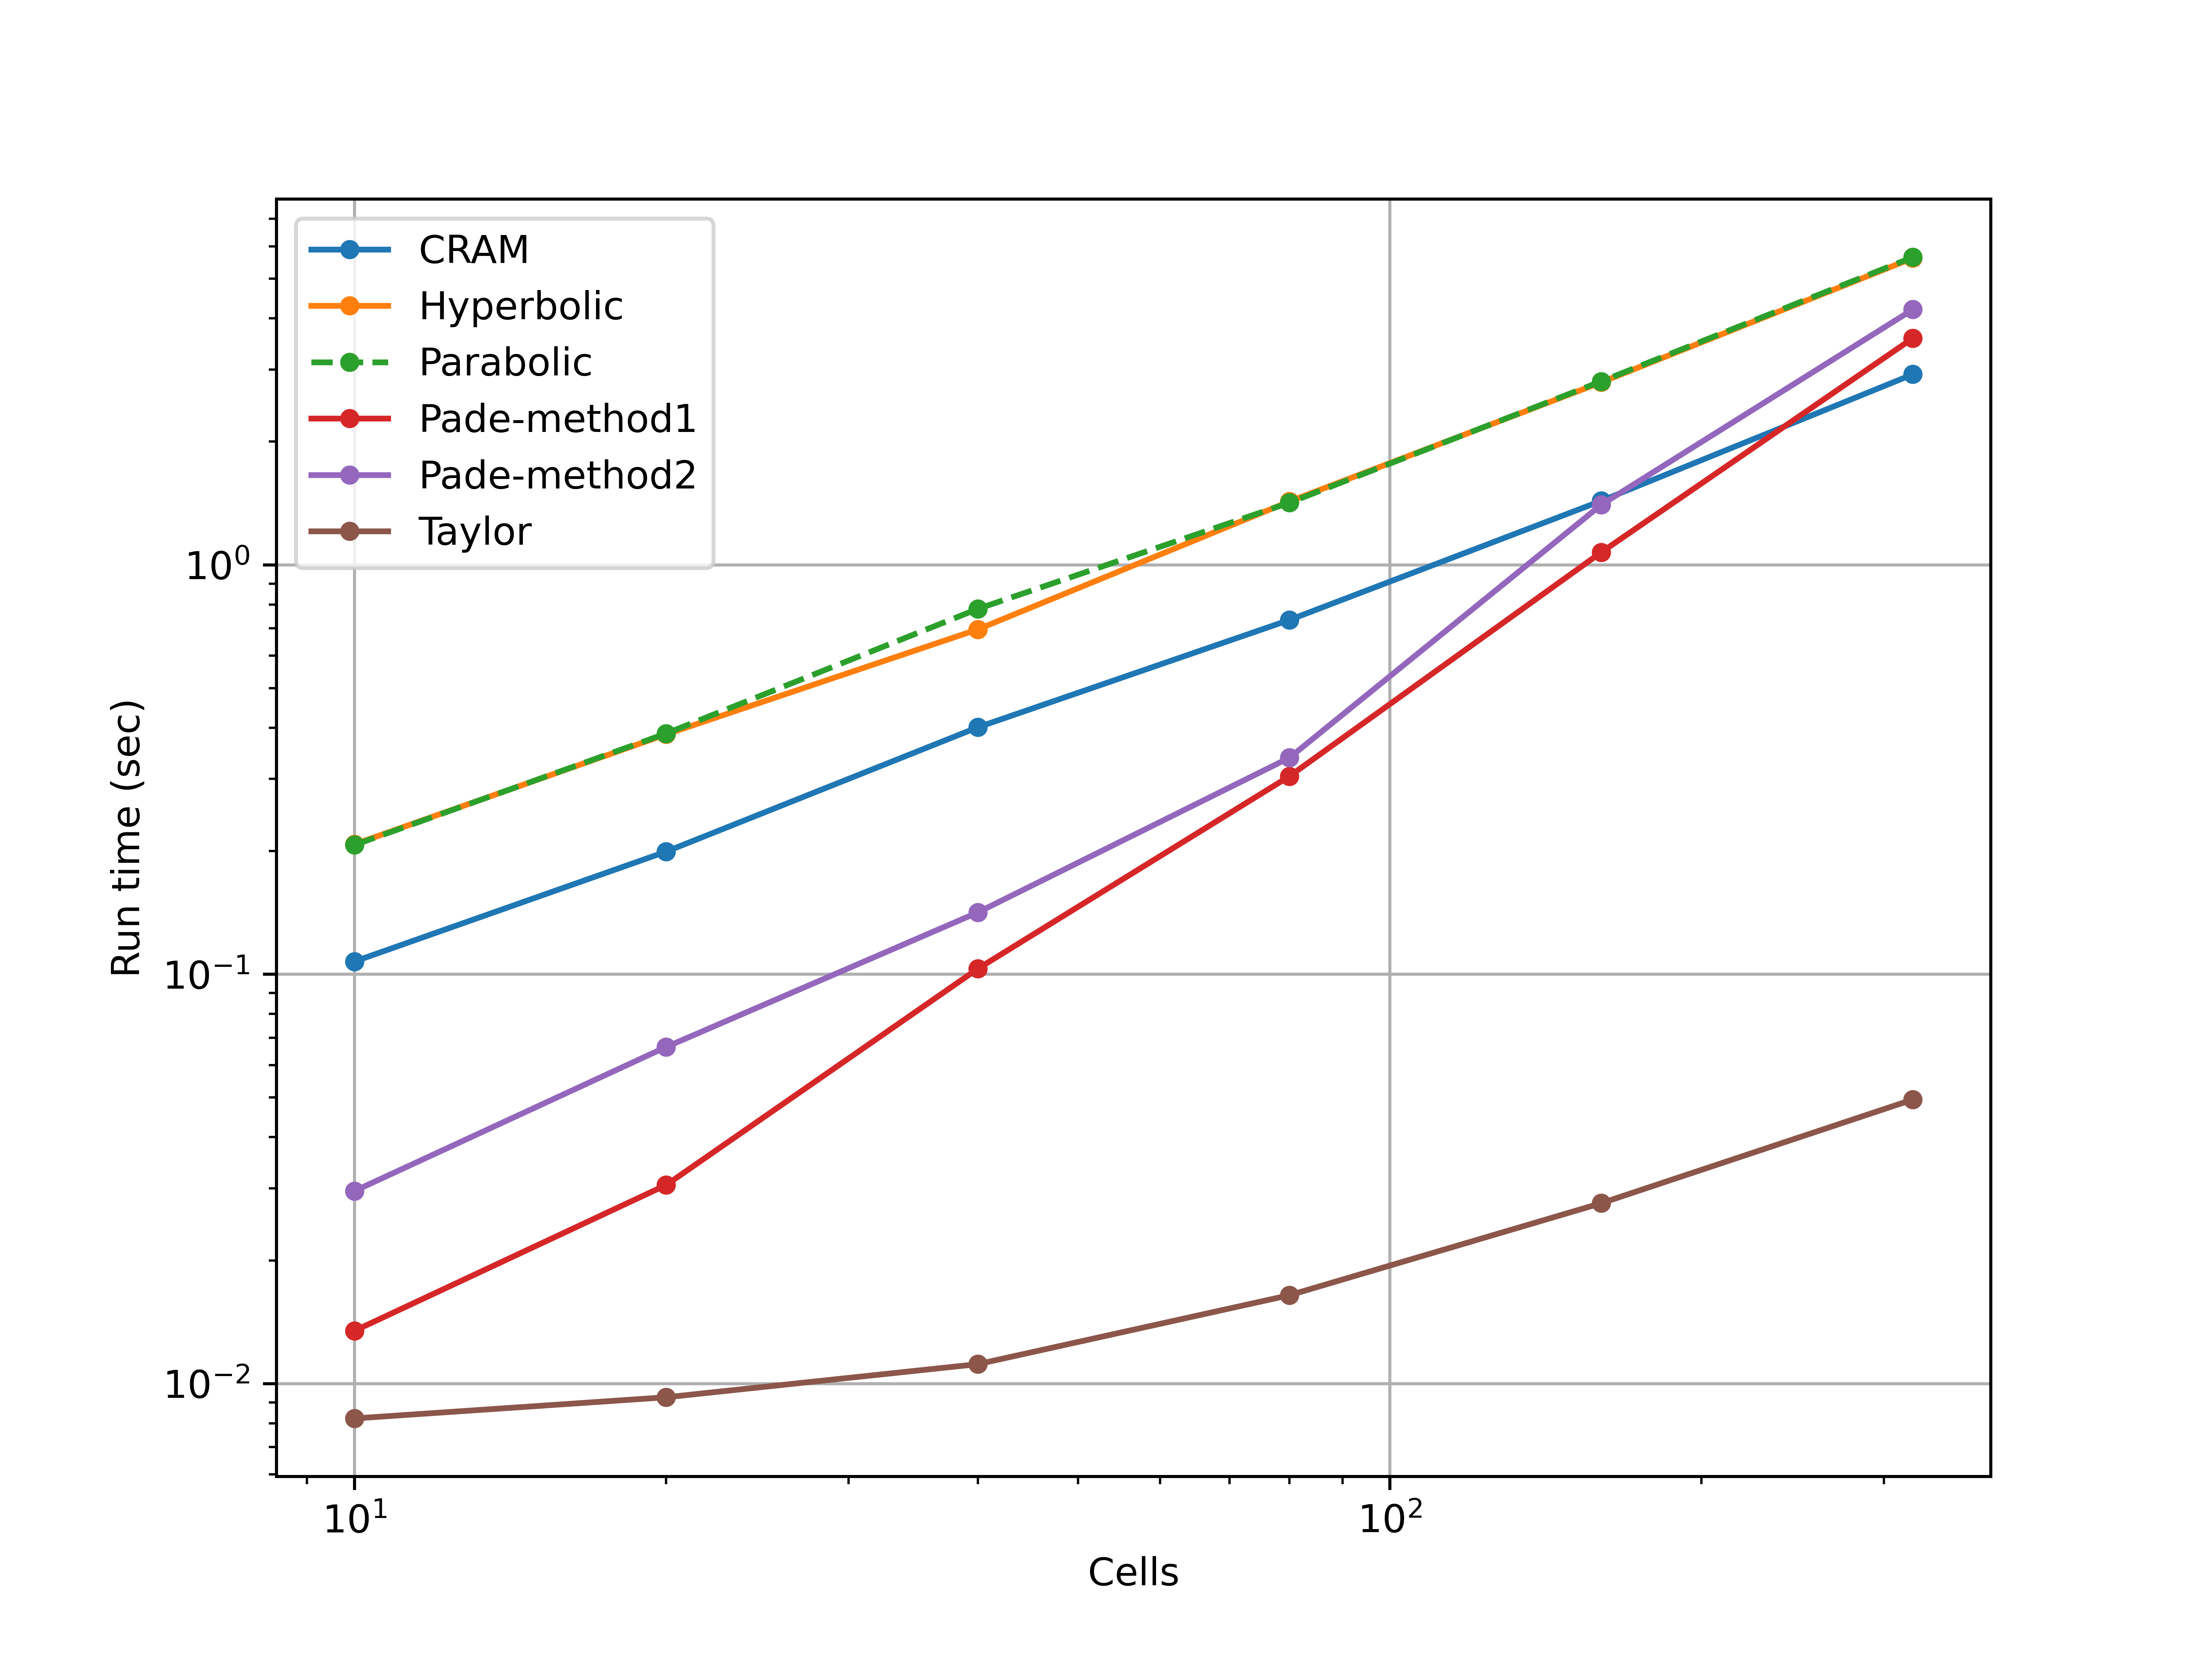
\includegraphics[width=6in]{images/chapter-5/progressionProblems/problem4/problem4Runtimes.png}
    \caption{Problem 4 average run times for each solver, dt = 0.01}
    \label{fig:problem4_runtimes}
\end{figure}

\clearpage

\subsection{Problem 5}
This problem consist on a convection-reaction problem with a single species represented by:

\begin{equation}
    \frac{\partial C}{\partial t} = -v\frac{\partial C}{\partial x} - \lambda C,
\end{equation}

\noindent on the domain $x \in [0,100]$, $t \in [0,20]$ where $v = 2$ and $\lambda = 0.01$. Subject to the following conditions:

\begin{equation}
    C(x, 0) = 1000, \quad C(0,t) = 1000, \quad \frac{dC}{dx}(100, t) = 0.
\end{equation}

\noindent This leads to the analytic solution:

\begin{equation}
C (x,t) = \begin{cases}
  C (x, 0) e^{-\frac{x \lambda _i}{v}}\ , & x < vt \\
  C (x, 0) e^{-t \lambda _i}\ , & x \ge vt
\end{cases}
\end{equation}

This problem is a 1D convection driven flow where the species decays at a constant rate. The solution to this leads to a function that is not smooth, causing the higher order flux limiter functions to reduced to first order accuracy. Figures \ref{fig:problem5_l1error_spatial_results} and \ref{fig:problem5_l1error_time_results} show results for each of the flux limiter functions for the E${}_{1}$ relative error for spatial and temporal discretization. Starting with figure \ref{fig:problem5_l1error_spatial_results}, each of the flux limiters show about the same convergence rate at the first order upwind function. This agrees with the previous statement about TVD schemes reducing to first order convergence rates for non smooth solutions. While the TVD schemes do not have second order convergence rates, they do increase the accuracy of the solution when compared to first order upwind. This is most prevalent with the Albada limiter, which does show are higher convergence rate with large number of cells and time steps. This limiter also maintains the lowest error for all test shown if figures \ref{fig:problem5_l1error_spatial_results} and \ref{fig:problem5_l1error_time_results}. Albada also benefits the most from increasing the number of time steps, this is easly seen in figure \ref{fig:problem5_l1error_time_results}. Figure \ref{fig:problem5_l1error_time_results} also shows that each of the other flux limiter functions are not greatly affected by increasing the number of time steps. For smaller spatial discretizations, increasing the number of time steps does slightly increase the accuracy of the other TVD schemes. Results using the E${}_{\infty}$ and E${}_{2}$ errors are found in Appendix \ref{appen:results} figures \ref{fig:problem5_linferror_spatial_results}, \ref{fig:problem5_linferror_time_results}, \ref{fig:problem5_l2error_spatial_results} and \ref{fig:problem5_l2error_time_results}. Figure \ref{fig:problem5_linferror_spatial_results} shows that the E${}_{\infty}$ error behaves a little worse than E${}_{1}$, showing different flux limiters achieve minimal error at higher spatial resolution. While Albada is still one of the best, it does not have the lowest error for higher spatial and temporal resolutions. The E${}_{2}$ error, shown in figure \ref{fig:problem5_l2error_spatial_results}, shows the same behavior as E${}_{1}$. The Albada limiter performs the best and is affected the most by increasing the number of time steps.  

Figure \ref{fig:problem5_l1error_fluxlimiter_convergence_rate} shows convergence rates as a function of time and space. Unlike problem 4, which showed minimal convergence rate in the bottom left corner, these results show the minimal to be in the top left. This corresponds to low spatial and temporal resolution. For each limiter function, the convergence rate is increased by increasing the number of time steps taken. Just as with figures \ref{fig:problem5_l1error_spatial_results} and \ref{fig:problem5_l1error_time_results}, figure \ref{fig:problem5_l1error_fluxlimiter_convergence_rate} shows the the Albada limiter has the highest convergence rate, reaching a sweet spot at 80 cells and 400 time steps. Figures \ref{fig:problem5_linferror_fluxlimiter_convergence_rate} and \ref{fig:problem5_l2error_fluxlimiter_convergence_rate} shows convergence rates for E${}_{\infty}$ and E${}_{2}$ errors. The $l_{\infty}$ error shows high convergence rates for for low cells and high time steps for all but the Albada and Min-Mod limiters. The E${}_{2}$ error shows high convergence rates for high time steps, generally reaching a plateau as the number of cells in increased.

Figure \ref{fig:problem5_l1error_coefficient_changes} shows how the problem behaves as a function of $v$ and $\lambda$. These coefficients are changed to induce and reaction or velocity dominated system. In a reaction dominated system, all of the flux limiter functions converge to a single point. This is because the accuracy of the solution is dominated by the integration of the reaction rate of the time interval. As the velocity is increased, the flux limiters begin to diverge to difference accuracy's. The Albada limiter diverges the most, decreasing the error 2 orders of magnitude below all the others. What is also interesting is that the error follows a hump shape, increasing up until it reaches a max value where the coefficient are the same. After this, the error decreases. This is also the point where the Albada separates from the rest. 

Figure \ref{fig:problem5_runtimes} show how each of the solvers scale with number of cells. On the log-log scale, the Cauchy and Taylor solvers scale linearly while the Pad\'e solvers begin low then increase to a point above the others. This indicates that the Pad\'e solvers scale much more poorly. As with problem 3, the Cauchy solvers did show instability. These instabilities were also remedied by increasing the order of the method and by adding substeps. 

\clearpage

\begin{figure}[p]
    \centering
    \includegraphics[width=6in]{images/chapter-5/progressionProblems/problem5/problem5E1ErrorWithSpace.png}
    \caption{Problem 5 relative E${}_{1}$ error with spatial discretization at various time steps}
    \label{fig:problem5_l1error_spatial_results}
\end{figure}

\clearpage

\begin{figure}[p]
    \centering
    \includegraphics[width=6in]{images/chapter-5/progressionProblems/problem5/problem5E1ErrorWithTime.png}
    \caption{Problem 5 relative E${}_{1}$ error with temporal discretization at various number of spatial cells}
    \label{fig:problem5_l1error_time_results}
\end{figure}

\clearpage

\begin{figure}[p]
    \centering
    \includegraphics[width=6in]{images/chapter-5/progressionProblems/problem5/problem5E1FluxLimiterConvergenceRate.png}
    \caption{Problem 5 flux limiter relative E${}_{1}$ spatial convergence rate using absolute error}
    \label{fig:problem5_l1error_fluxlimiter_convergence_rate}
\end{figure}

\clearpage

\begin{figure}[p]
    \centering
    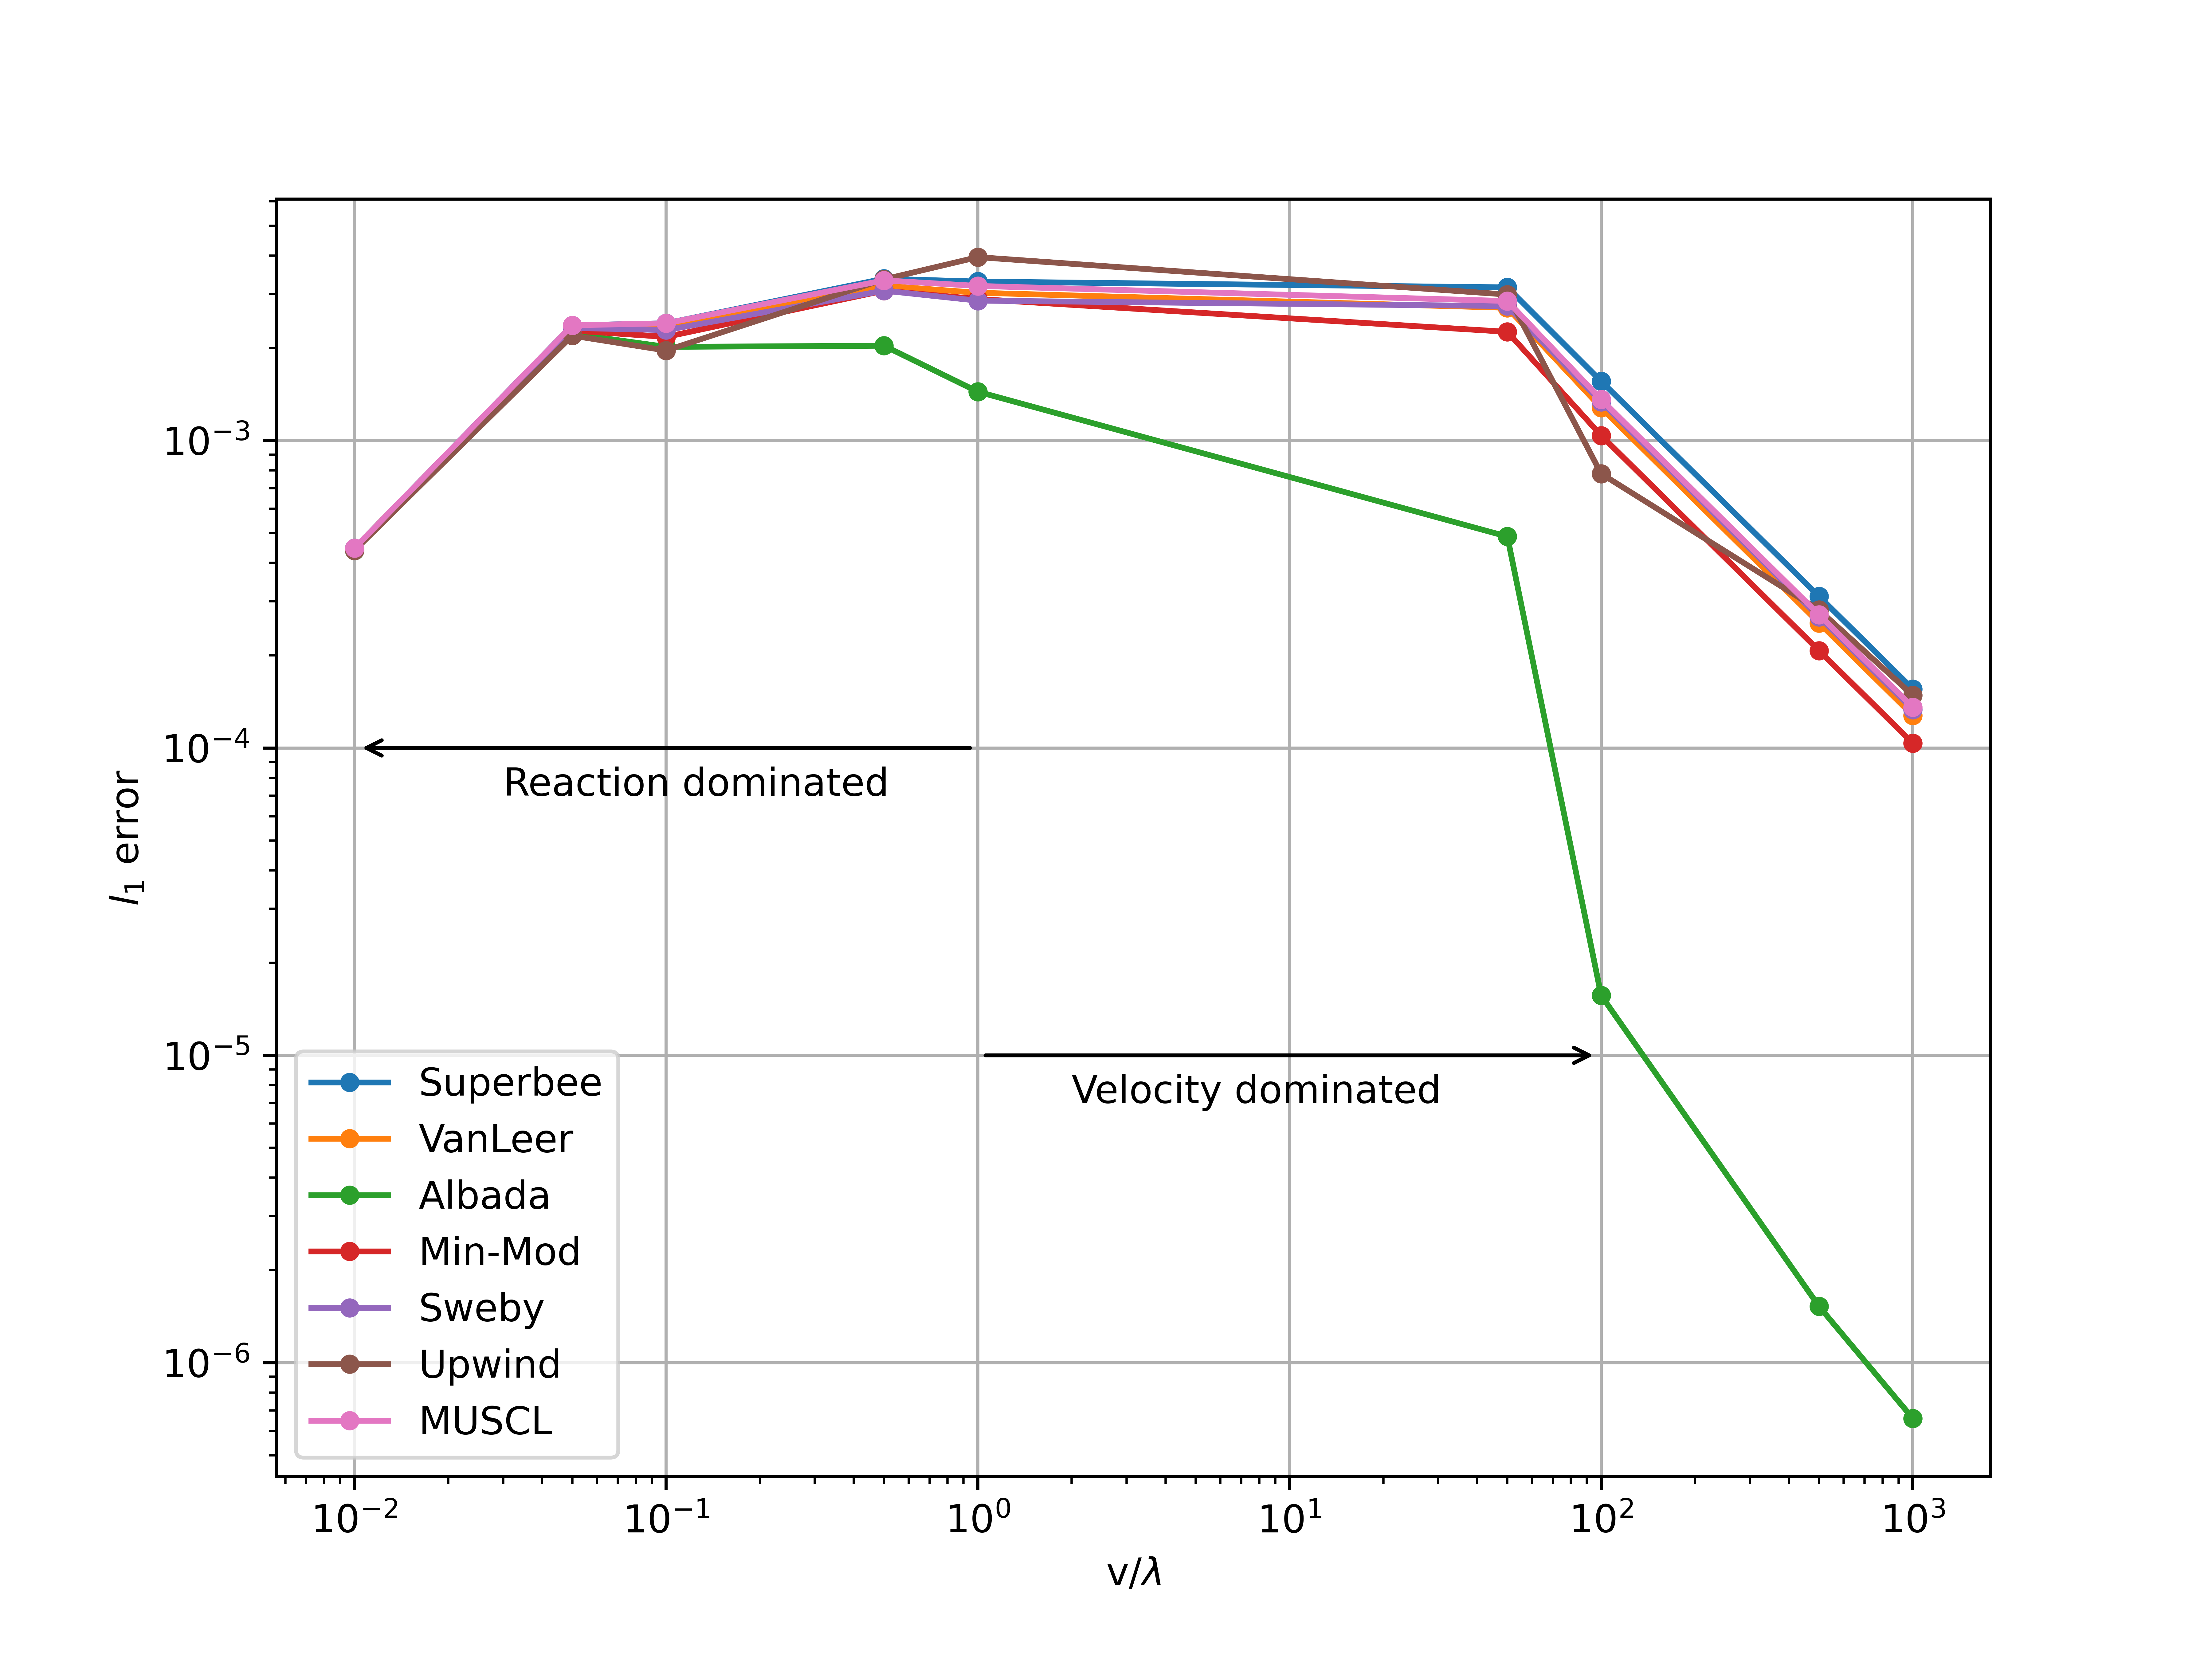
\includegraphics[width=6in]{images/chapter-5/progressionProblems/problem5/problem5CoefficientChanges.png}
    \caption{Problem 5 flux limiter relative E${}_{1}$ behavior with coefficient changes using absolute error}
    \label{fig:problem5_l1error_coefficient_changes}
\end{figure}

\clearpage

\begin{figure}[p]
    \centering
    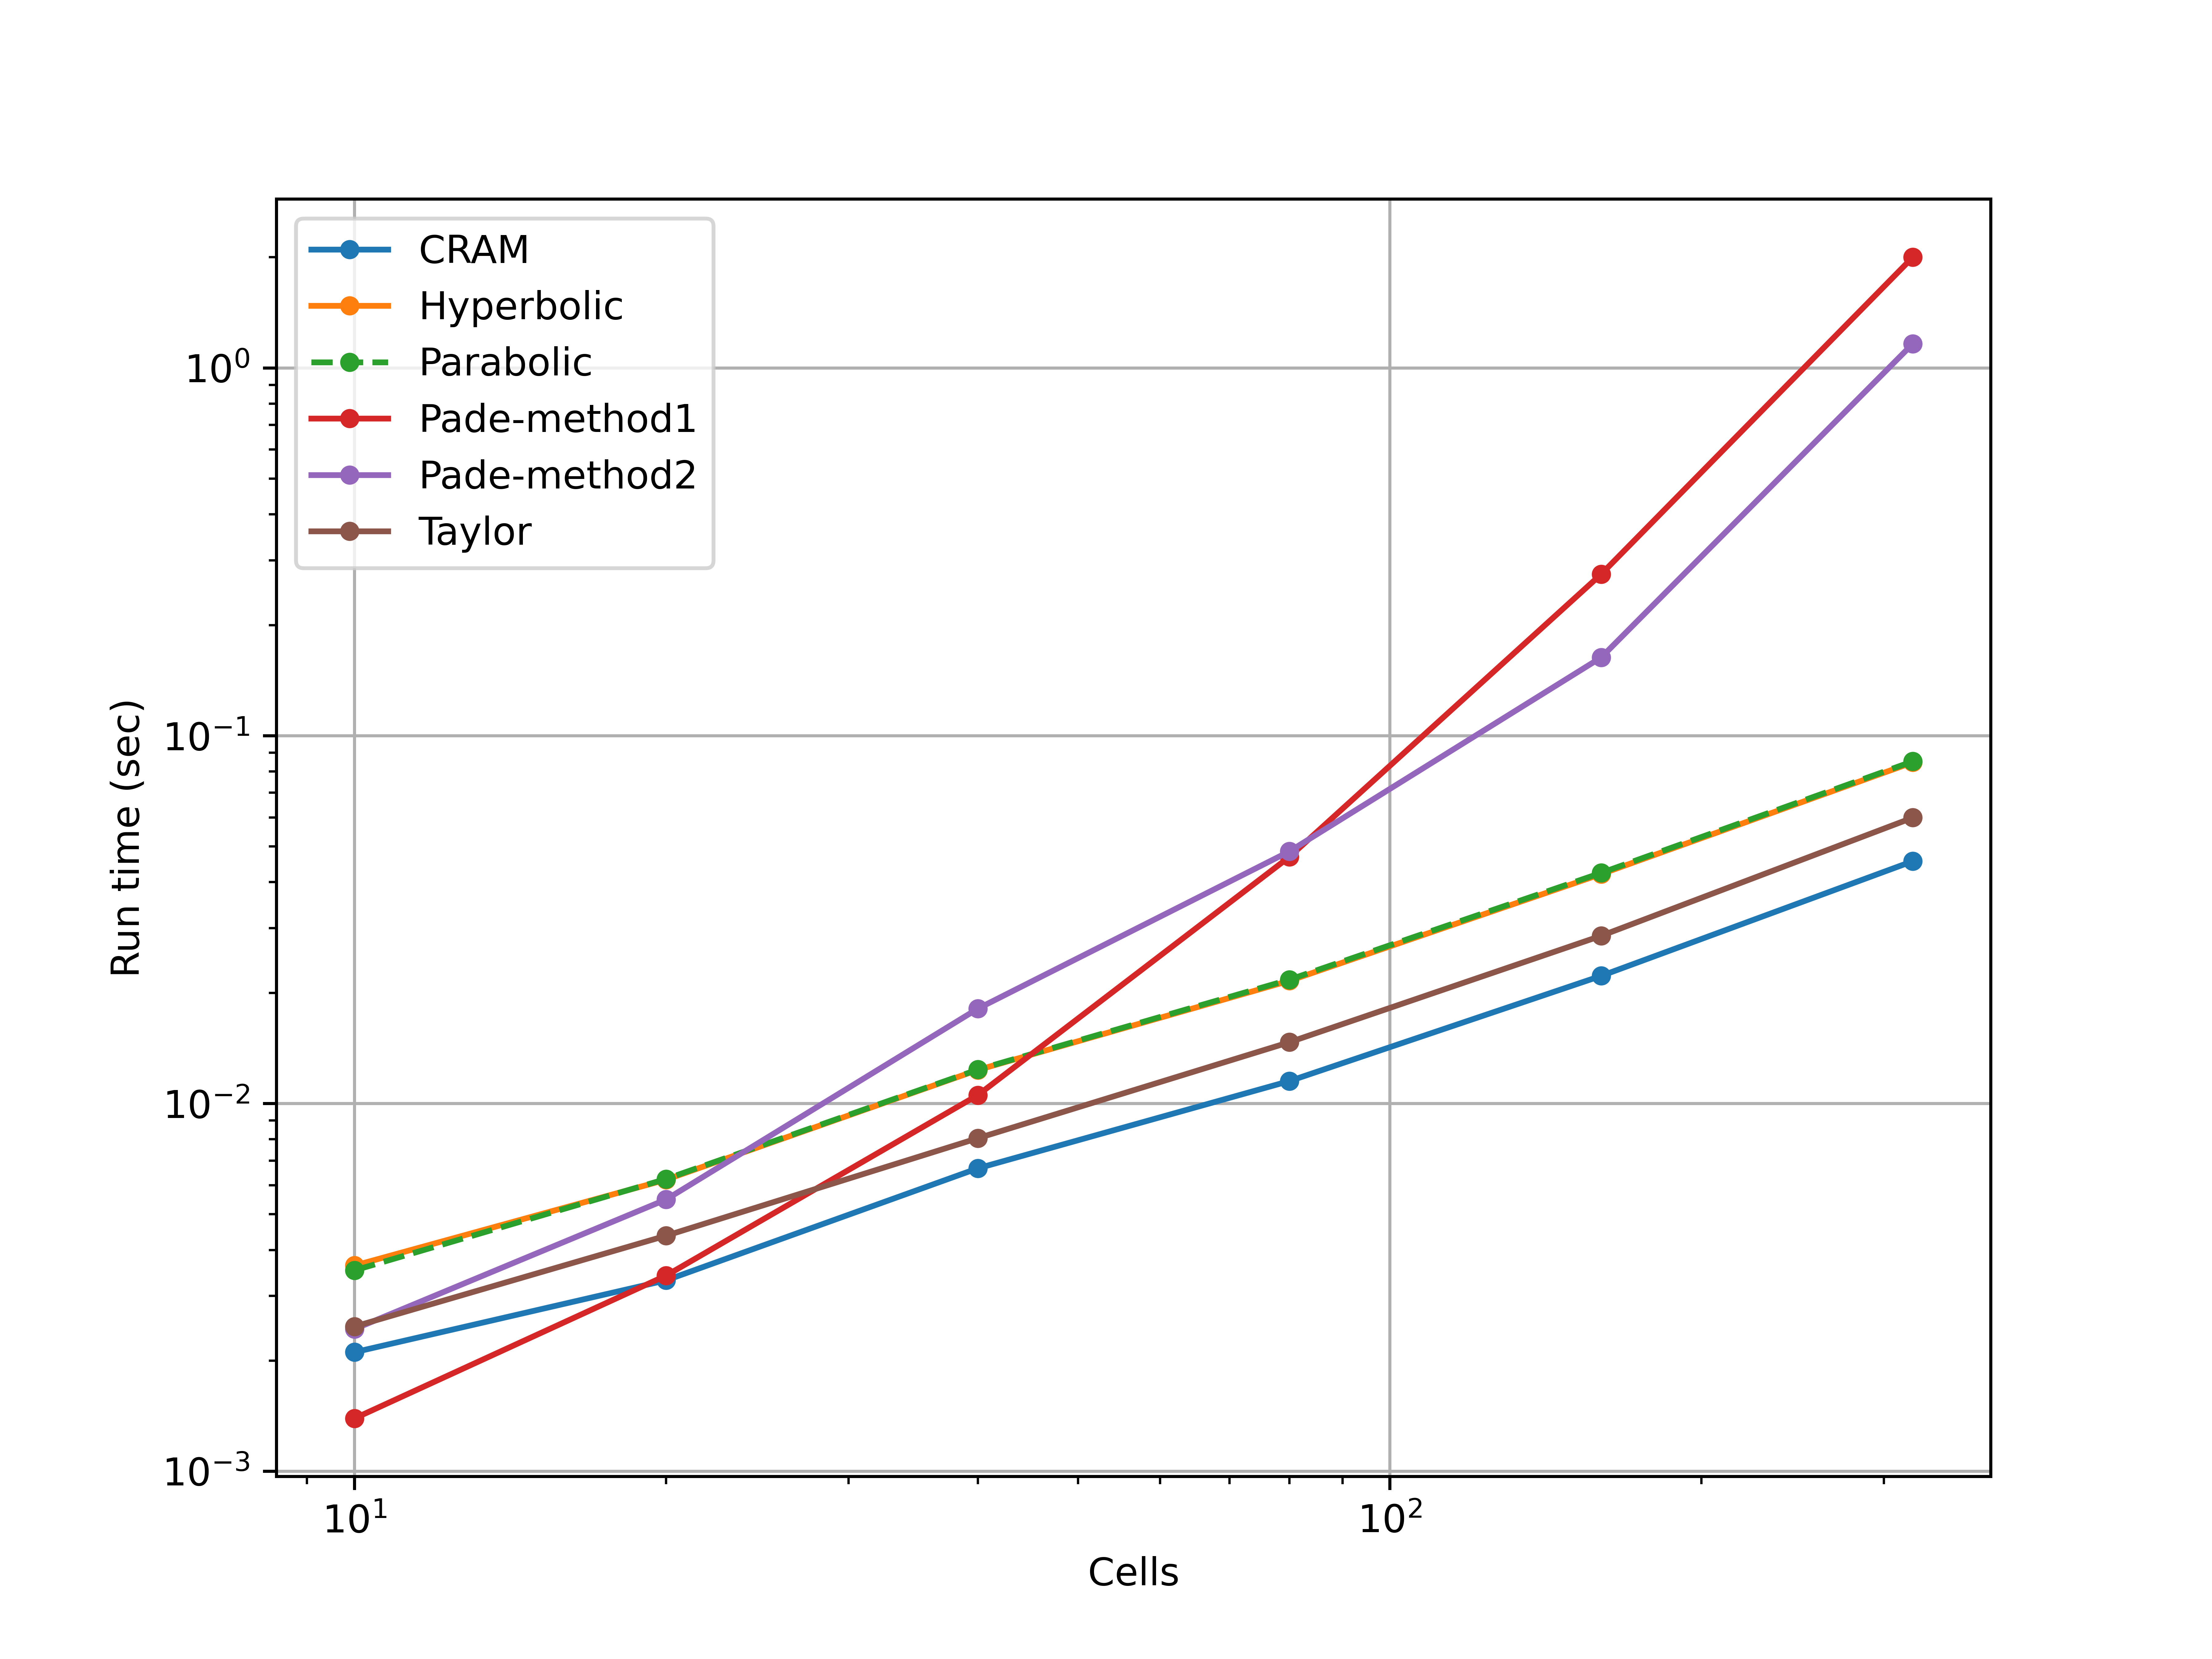
\includegraphics[width=6in]{images/chapter-5/progressionProblems/problem5/problem5Runtimes.png}
    \caption{Problem 5 average run times for each solver, dt = 0.1}
    \label{fig:problem5_runtimes}
\end{figure}

\clearpage

\subsection{Problem 6}
This is an extension of problem 6 with two species, one that exist in the liquid and one on the wall. The species in the liquid transports and depositions on the wall where it sticks and does not move. In libowski this is accomplished by excluding the loop which adds the convection contribution to the wall species. This system is represented by:

\begin{equation}
\setlength{\jot}{15pt}
\begin{split}
    &\frac{\partial C_{l}}{\partial t} = -v\frac{\partial C_{l}}{\partial x} - \frac{kA}{V} C_{l}, \\
    &\frac{\partial C_{w}}{\partial t} = \frac{kA}{V} C_{l},
    \label{eq:problem6}
\end{split}
\end{equation}

\noindent on the domain $x \in [0,100]$, $t \in [0, 20]$ where $v = 2$ and $kA/V = \lambda = 0.01$. Subject to the following conditions:

\begin{equation}
\setlength{\jot}{15pt}
\begin{split}
    C_{l}(x, 0) = 1000, \quad C_{l}(0,t) = 1000, \quad \frac{dC_{l}}{dx}(100, t) = 0, \\
    C_{w}(x, 0) = 0, \quad C_{w}(0,t) = 0, \quad \frac{dC_{l}}{dx}(100, t) = 0. \\
\end{split}
\end{equation}

\noindent Let $\lambda = kA/V$, equation \ref{eq:problem6} the following solution:

\begin{equation}
C_{l} (x,t) = \begin{cases}
  C_{l} (x, 0) e^{-\frac{x \lambda _i}{v}}\ , & x < vt \\
  C_{l} (x, 0) e^{-t \lambda _i}\ , & x \ge vt
\end{cases}
\end{equation}

\begin{equation}
C_{w} (x,t) = \begin{cases}
  C_{l} (x, 0) \Big( 1 - e^{-\frac{x \lambda _i}{v}} + \lambda \big(t - x/v\big)e^{-\lambda x/v} \Big)\ , & x < vt \\
  C_{l} (x, 0) \Big( 1 - e^{-t \lambda _i}\Big)\ , & x \ge vt
\end{cases}
\end{equation}

This problem is conducted in the same manor as problem 4 and 5. But unlike problem 4, this problem has a discontinuous solution. Figures \ref{fig:problem6_l1error_spatial_results} and  \ref{fig:problem6_l1error_time_results} shows results for the E${}_{1}$ error as a function of time and space. These results shows the same behavior for each of the flux limiters that was shown in problem 4. The only difference is the error is slightly higher in this problem. Again, the Albada flux limiter showes the lowest over all error and does show the most improvment from increasing the number of time steps. 

\clearpage

\begin{figure}[p]
    \centering
    \includegraphics[width=6in]{images/chapter-5/progressionProblems/problem6/problem6E1ErrorWithSpace.png}
    \caption{Problem 6 relative E${}_{1}$ error with spatial discretization at various time steps}
    \label{fig:problem6_l1error_spatial_results}
\end{figure}

\clearpage

\begin{figure}[p]
    \centering
    \includegraphics[width=6in]{images/chapter-5/progressionProblems/problem6/problem6E1ErrorWithTime.png}
    \caption{Problem 6 relative E${}_{1}$ error with temporal discretization at various number of spatial cells}
    \label{fig:problem6_l1error_time_results}
\end{figure}

\clearpage

\begin{figure}[p]
    \centering
    \includegraphics[width=6in]{images/chapter-5/progressionProblems/problem6/problem6E1FluxLimiterConvergenceRate.png}
    \caption{Problem 6 flux limiter relative E${}_{1}$ spatial convergence rate using absolute error}
    \label{fig:problem6_l1error_fluxlimiter_convergence_rate}
\end{figure}

\clearpage

\begin{figure}[p]
    \centering
    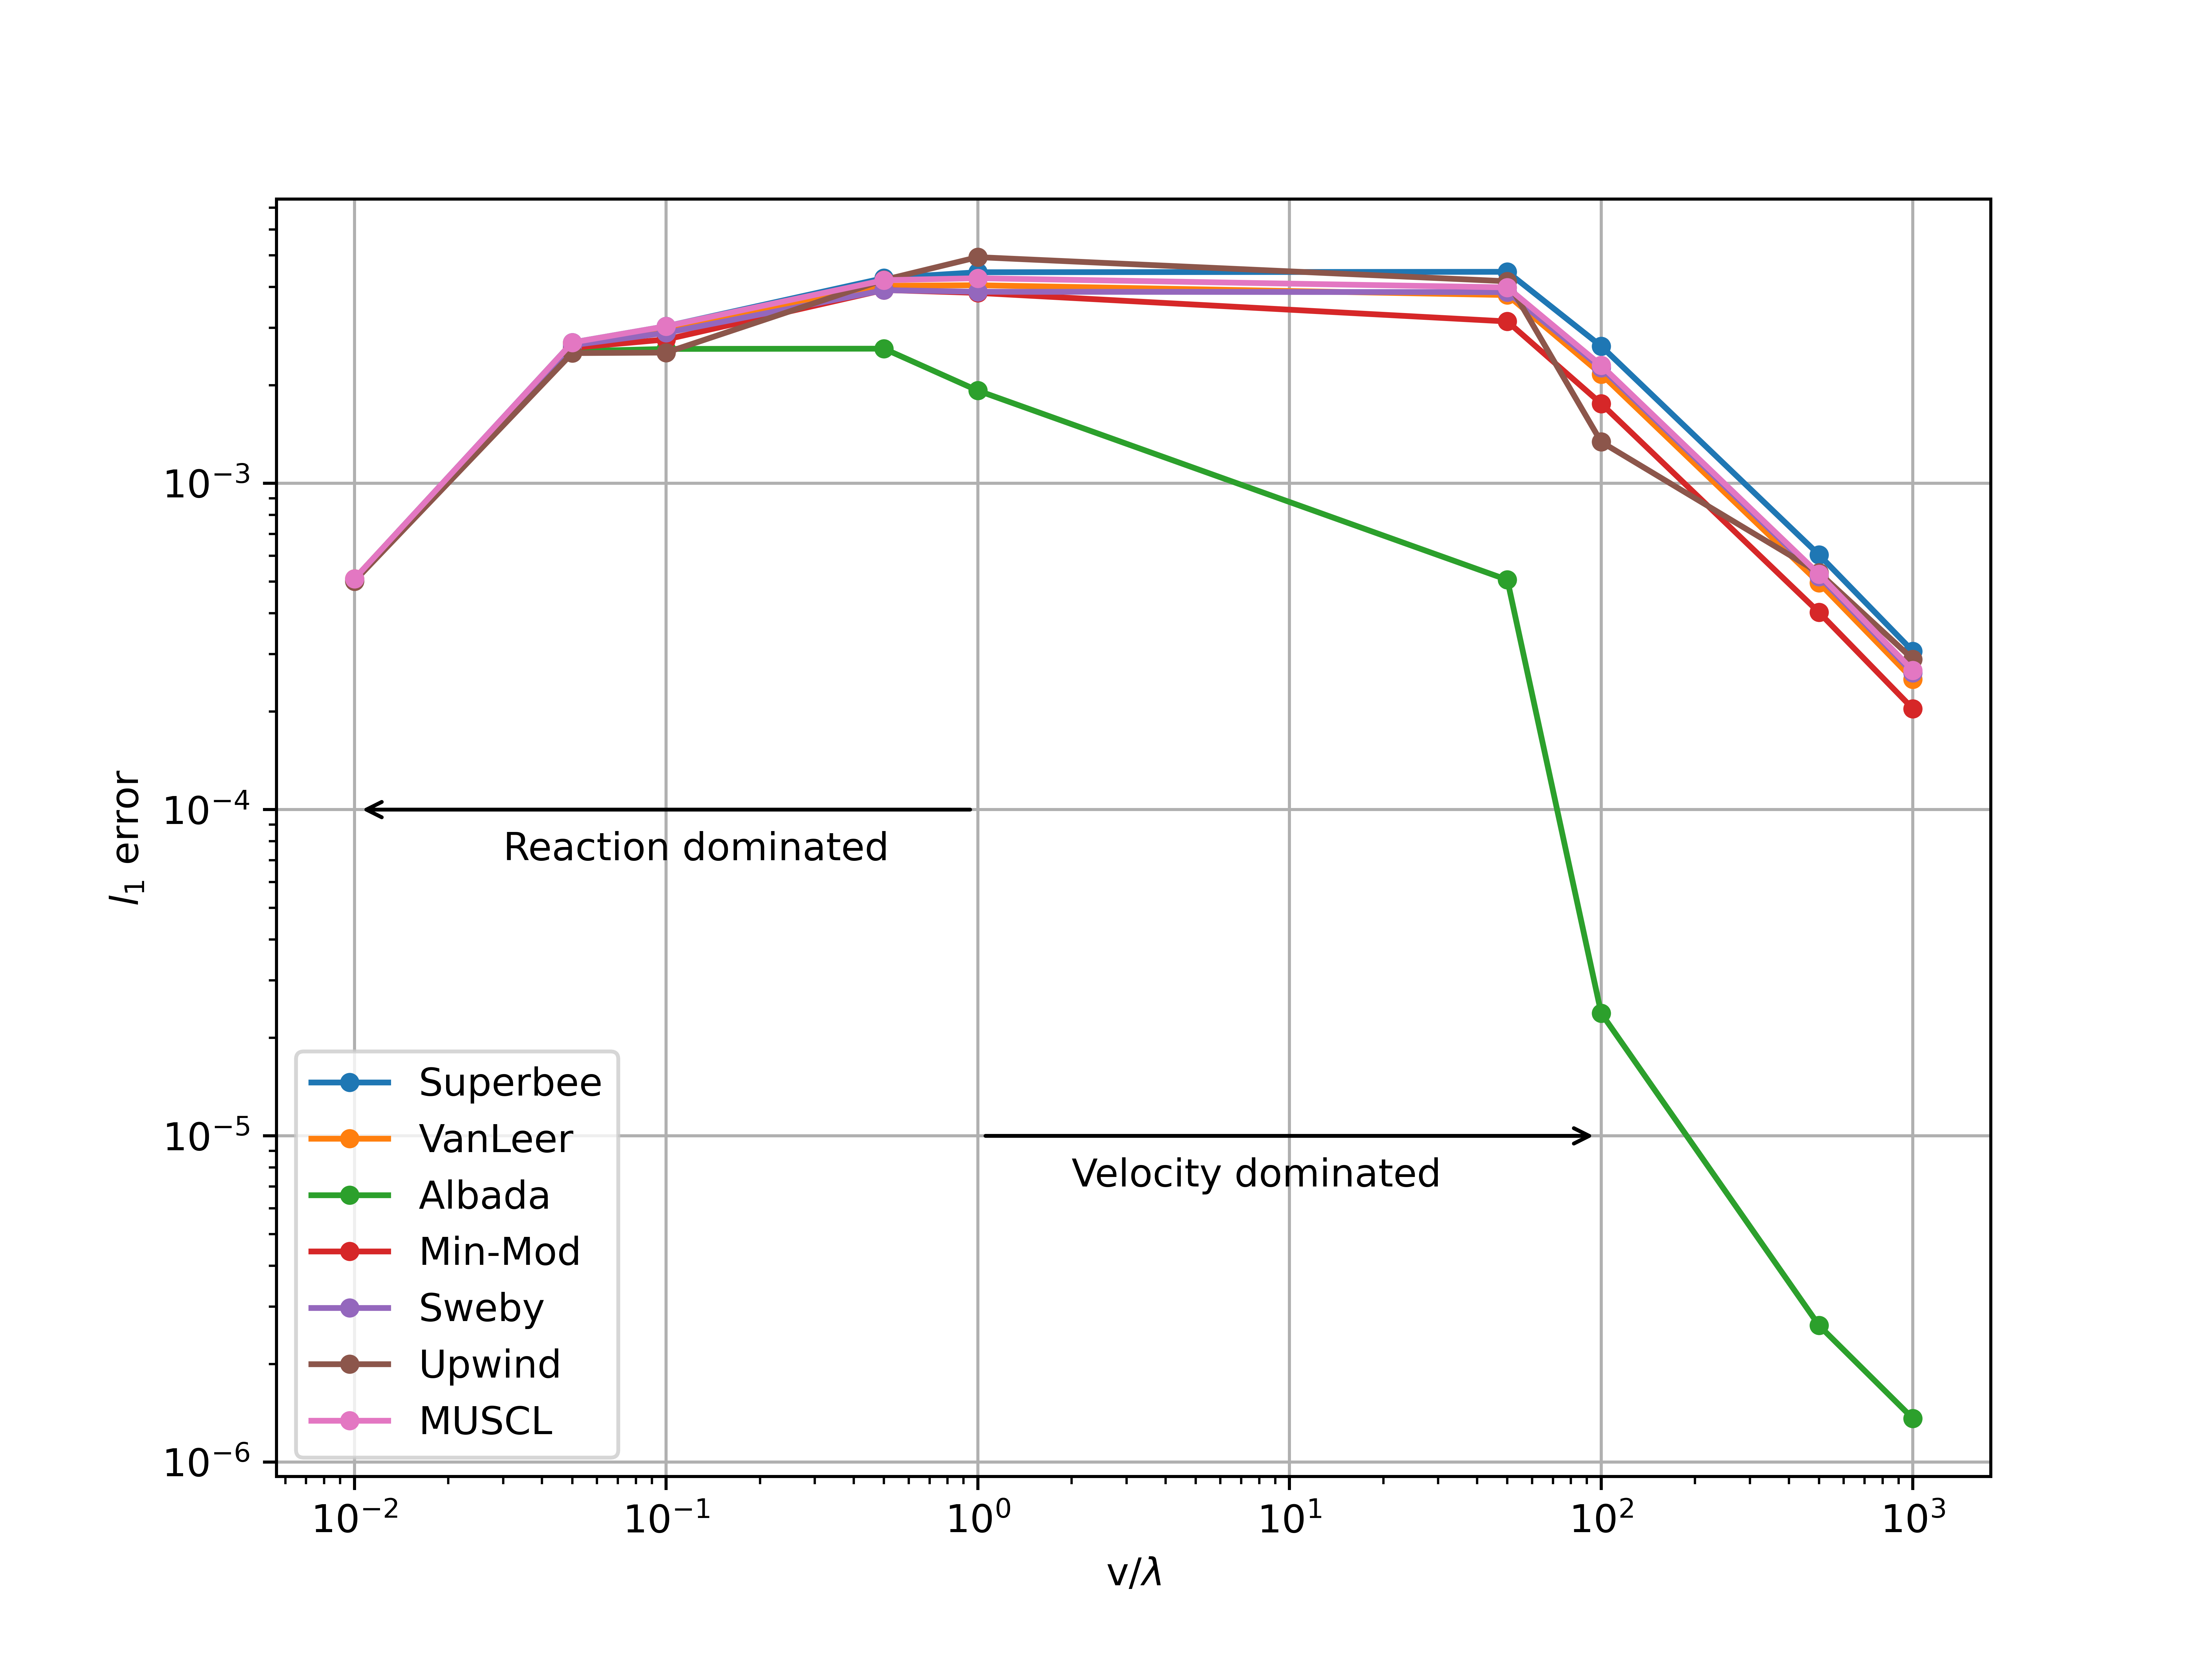
\includegraphics[width=6in]{images/chapter-5/progressionProblems/problem6/problem6CoefficientChanges.png}
    \caption{Problem 6 flux limiter relative E${}_{1}$ behavior with coefficient changes using absolute error}
    \label{fig:problem6_l1error_coefficient_changes}
\end{figure}

\clearpage

\begin{figure}[p]
    \centering
    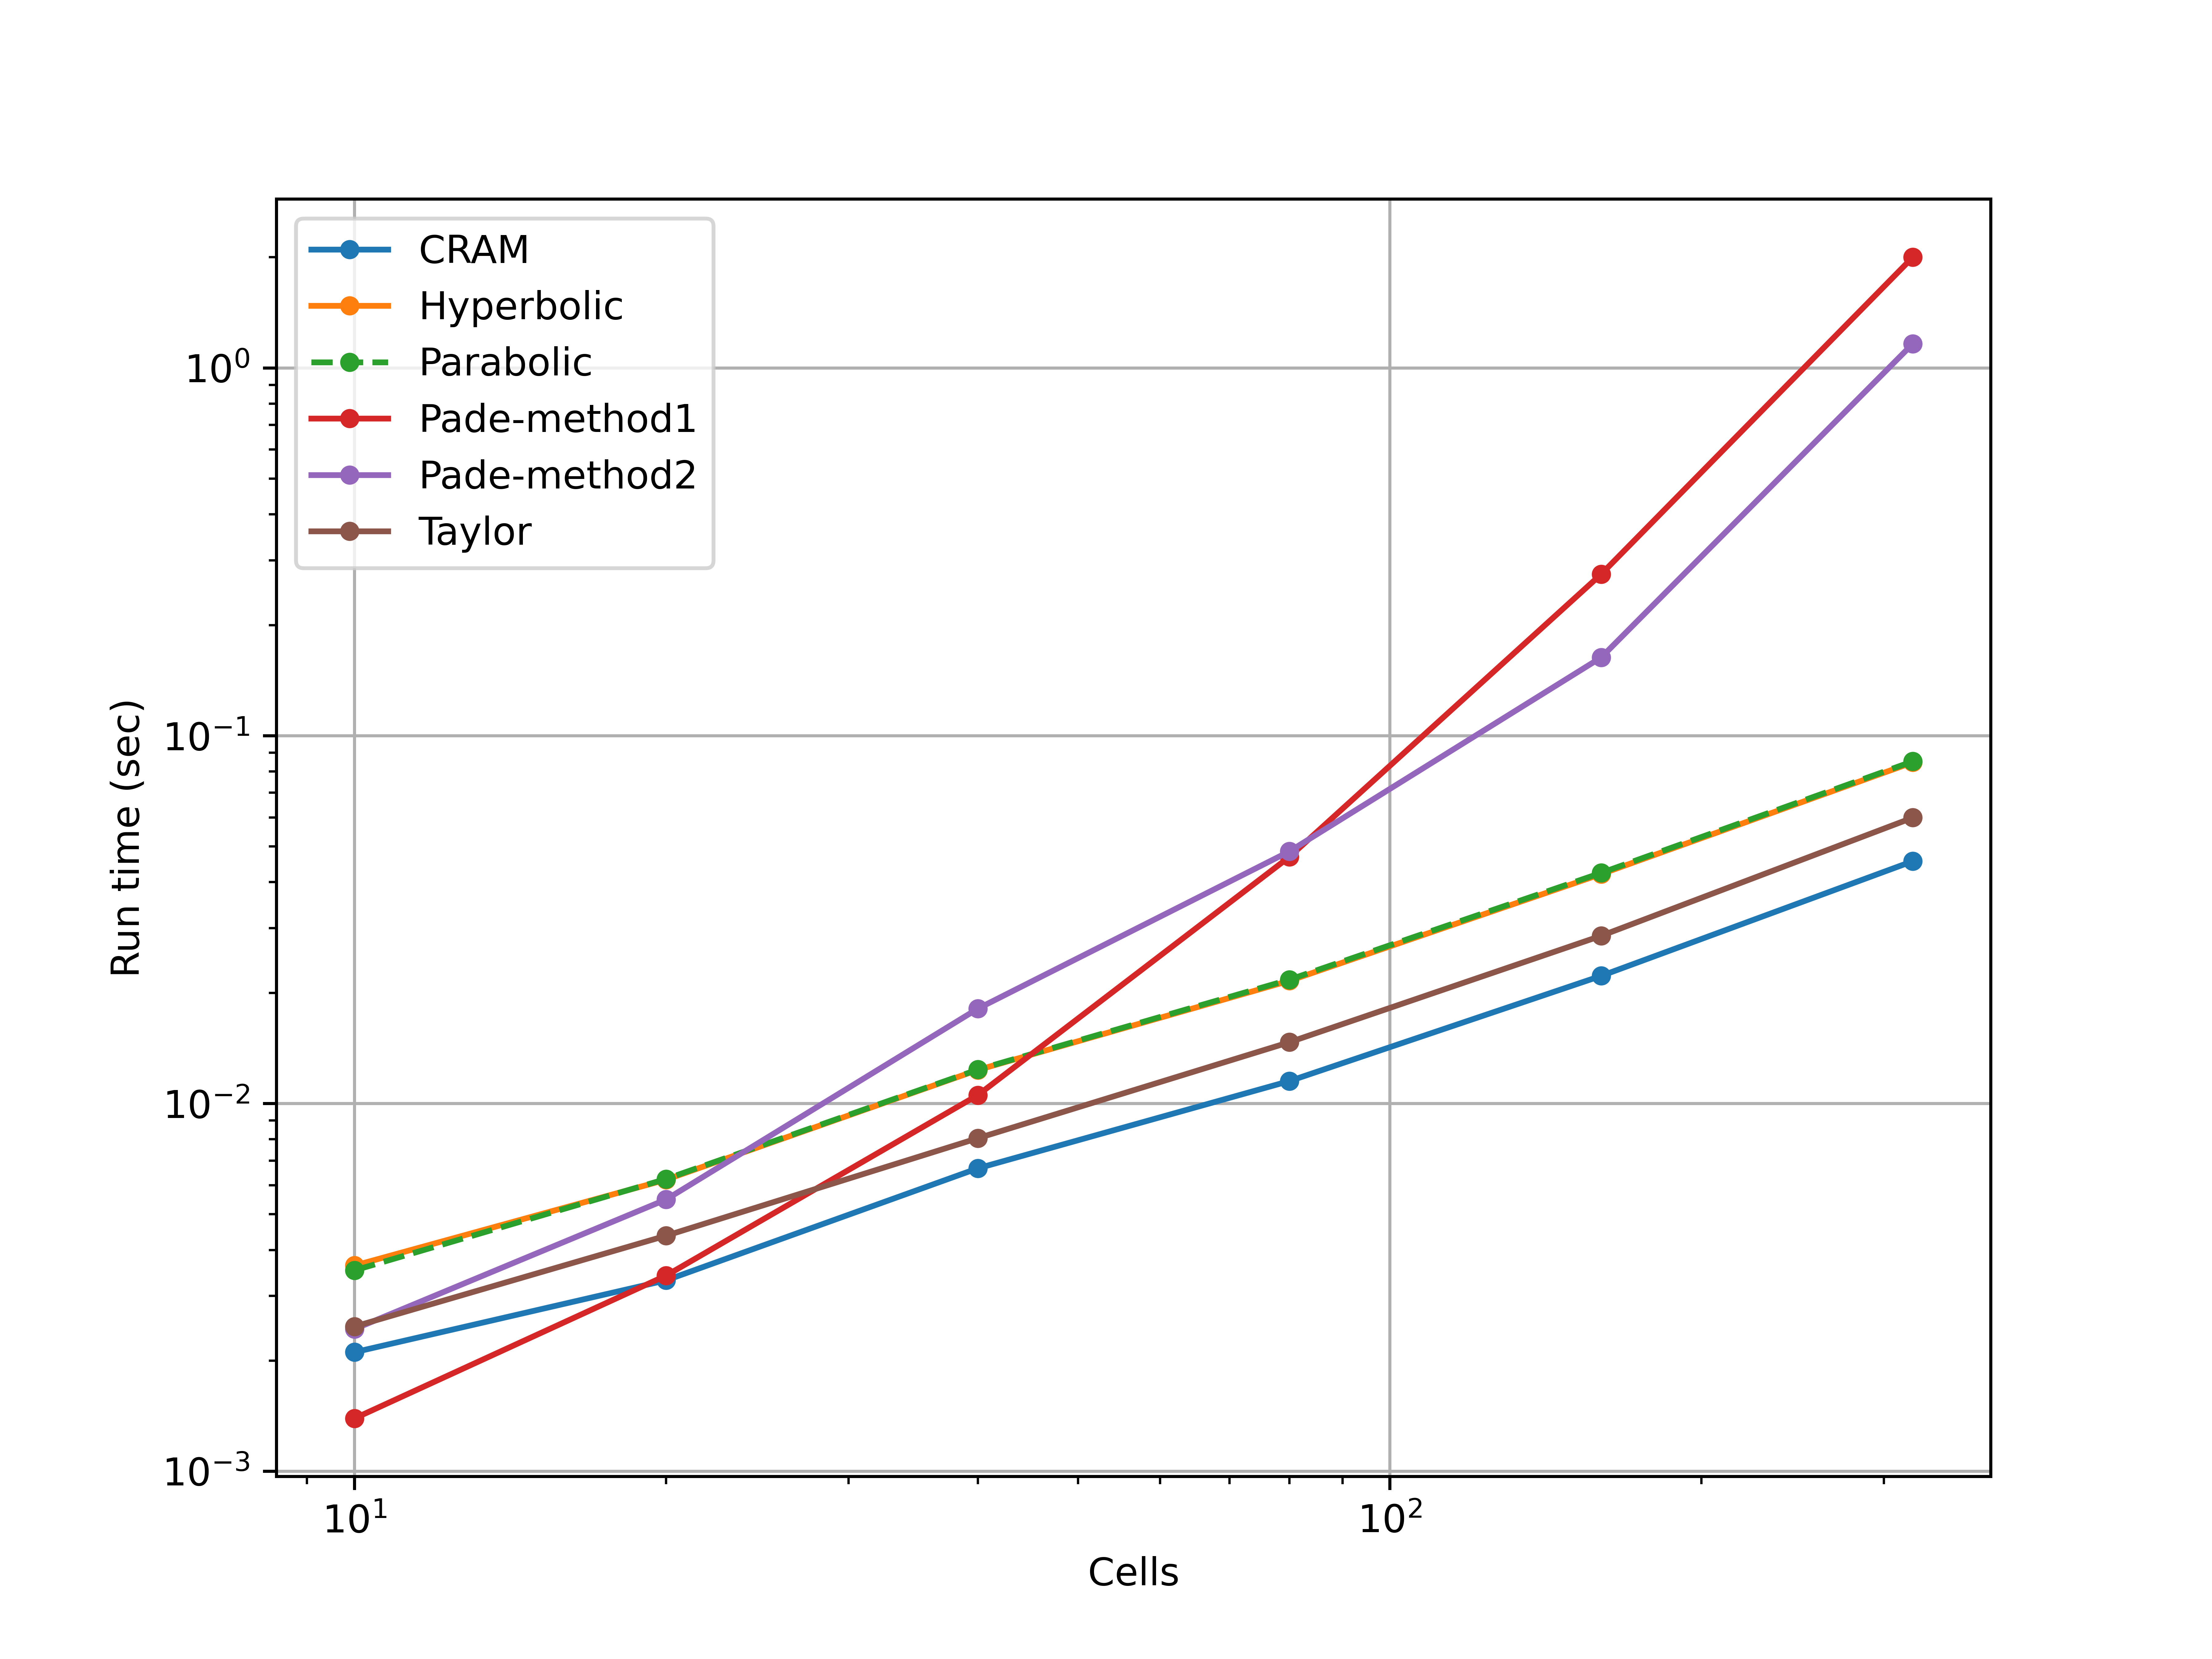
\includegraphics[width=6in]{images/chapter-5/progressionProblems/problem5/problem5Runtimes.png}
    \caption{Problem 5 average run times for each solver, dt = 0.1}
    \label{fig:problem5_runtimes}
\end{figure}

\clearpage

\subsection{Problem 7}
This problem models the primary uranium isotopes along with Pu-239 and Np-239 in a system which contains a neutron flux. Coefficients in the transition matrix include source and sink terms from both neutron induced reactions and radioactive decay. This system is represented by:


\begin{equation}
\frac{d C_i}{dt} = \sum^9_{j = 1} A_{ij} C_j (x, t)
\end{equation}

\begin{equation}
i = \begin{dcases}
  1 , & \text{$^{233}$U}  \\
  2 , & \text{$^{234}$U}  \\
  3 , & \text{$^{235}$U}  \\
  4 , & \text{$^{236}$U}  \\
  5 , & \text{$^{237}$U}  \\
  6 , & \text{$^{238}$U}  \\
  7 , & \text{$^{239}$U}  \\
  8 , & \text{$^{239}$Pu} \\
  9 , & \text{$^{239}$Np} \\
\end{dcases}
\end{equation}

\noindent On the domain from $t \in [0, 500]$ subject to the following neutron flux $\phi = 1e13$. Each isotope is given an initial concentration of $C_{i, 0} = 1e10$. The transition matrix is built using information from the SCALE ORIGEN library. The analytical solution is given by the exponential of the transition matrix:

\begin{equation}
   \boldsymbol{C}(t) = e^{\boldsymbol{A}t}, 
\end{equation}

\noindent where $\boldsymbol{C}$ is a vector of isotope concentrations. The solution is calculated using in MATLAB using the method previously described. 


\subsection{Problem 8}
This is an extension of problem 9 but for a fictitious "pipe" reactor which allows for the flow of isotopes due to a velocity. This is represented by:

\begin{equation}
\frac{d C_i}{dt} = -v\frac{\partial C_{i}}{\partial x} + \sum^9_{j = 1} A_{ij} C_j (x, t)
\end{equation}

\begin{equation}
i = \begin{dcases}
  1 , & \text{$^{233}$U}  \\
  2 , & \text{$^{234}$U}  \\
  3 , & \text{$^{235}$U}  \\
  4 , & \text{$^{236}$U}  \\
  5 , & \text{$^{237}$U}  \\
  6 , & \text{$^{238}$U}  \\
  7 , & \text{$^{239}$U}  \\
  8 , & \text{$^{239}$Pu} \\
  9 , & \text{$^{239}$Np} \\
\end{dcases}
\end{equation}

\noindent On the domain $x \in [0, 400]$, $t \in [0, 500]$ where $v = 25$ and $\phi(x) = 1e13$. Subject to the periodic boundary conditions:

\begin{equation}
    C_{i}(0,t) = C_{i}(400,t).
\end{equation}

\section{Case Studies}
The following are a selection of case studies which aim to explore libowskis' accuracy and performance with problems which come up in modeling MSRs. 

\subsection{Neutron precursors}
This problem examines a convection-driven flow with the 6 neutron precursor groups, as shown in Eqs. (\ref{eq:problem3}) and (\ref{eq:problem3flux}): 

\begin{equation}
\frac{\partial C_{i}}{\partial t} = -v_{x}\frac{\partial C_{i}}{\partial x} - v_{y}\frac{\partial C_{i}}{\partial y} + \beta_{i} \Psi (x, y) -\lambda_i C_{i},
\label{eq:problem3}
\end{equation}

\begin{equation}
\Psi (x, y) = \begin{cases}
  \psi _0 \sin\left(\frac{\pi x}{50}\right)\sin\left(\frac{\pi y}{100}\right) , x \in [0,50], y \le 100 \\
  0\ , \text{otherwise},
  \label{eq:problem3flux}
\end{cases}
\end{equation}

\noindent where $i \in [1,6]$, $x \in [0, 50]$, $y \in [0, 400]$, $t \in [0, 60]$, $v_{x} = 0$, and $v_{y} = 25$, subject to the following boundary conditions:

\begin{equation}
    C_{i}(x,0) = C_{i}(x,400), \quad \frac{dC_{i}}{dx}(0,y) = 0, \quad \frac{dC_{i}}{dx}(50, y) = 0.
\end{equation}

Coefficients for the system are shown in Table \ref{tab:precursorCoeffs} \cite{ott1985}. 
Each precursor had the same initial condition of zero, and the source term for each precursor was scaled in the x and y directions by the sine function. The spatial domain was modeled to mimic an MSR with a core region extending from $y \in [0,100]$ and $x \in [0,50]$, with a core exterior loop modeled from $y \in [100, 400]$. 

\begin{table}[h!]
   \caption{\label{tab:precursorCoeffs} Parameters for Neutron Precursors}
   \centering
   \begin{tabular}{lll}
   \hline
   Group & $\lambda$ & $\beta$ \\
   \hline
   1 & 0.0127 & 0.0006 \\
   2 & 0.0317 & 0.00364 \\
   3 & 0.115 & 0.00349 \\
   4 & 0.311& 0.00628 \\
   5 & 1.4 & 0.00179\\
   6 & 3.87 & 0.0007 \\
   \hline
   \end{tabular}
\end{table}     

While there is no analytic solution for this example problem, a reference solution was generated in Matlab using the symbolic tool box to solve for the matrix exponential. A small, spatially discretized problem was set up with 5 cells in the x direction and 20 in the y direction. The transition matrix that was built was then exported to Matlab, and the matrix exponential was solved at various times and saved as the reference solution. While the spatial accuracy was not tested in this case, this method will access the accuracy of each matrix exponential algorithm. To further simplify the problem, the first-order upwind difference scheme was applied to the convective flux.

One important feature for many of these solvers was the location of the eigenvalues for the transition matrix. The spectrum was calculated using the Matlab symbolic tool box and is plotted in Figure \ref{fig:spectrum_neutron_precursors} for dx = 10, dy = 20, and various values of dt. Figure \ref{fig:spectrum_neutron_precursors} show 6 elliptical rings, one at each dt, each one representing a precursor group. For a given time step size, the eigenvalues shifted along lines with slopes that are the ratio of their real and imaginary parts \cite{pusaAccruacy2013}. For a system in which the eigenvalues are located in a region where solutions based on Cauchy's integral break down, these eigenvalues can be shifted into a region where the solutions hold. Figure \ref{fig:spectrum_neutron_precursors} shows how changing the time step size can shrink the real and imaginary parts of the eigen spectrum.

\begin{figure}[htbp]
    \centering
    \includegraphics[width=3.5in]{images/neutronPrecursorEigenValues.png}
    \caption{Spectrum for the Neutron Precursors}
    \label{fig:spectrum_neutron_precursors}
\end{figure}


%\subsubsection{Accuracy as a function of substepping}
To understand how sub-stepping can work to improve the accuracy of a Cauchy-based solver, the neutron precursors problem was computed at 10-second time step intervals. The location of the eigenvalues is a function of the ratio $v_{x}/dx$ in the transition matrix; therefore, at the prescribed discretization, this ratio was manipulated by changing the flow velocity. For each Cauchy solver, the eigenvalues at two different flow velocities, 25 cm/s ($v_{x}/dx = 2.5$) and 60 cm/s ($v_{x}/dx = 6$), are shown in Figure \ref{fig:neturonprecursor_cauchy_eigenvalues}. As shown in Figure \ref{fig:neturonprecursor_cauchy_eigenvalues}, as the ratio increased, so did the spread of the eigenvalues on the real and imaginary axis. This led to a limitation of the velocity to discretization size for convection problems when using Cauchy solvers. One solution, which is also shown in Figure \ref{fig:neturonprecursor_cauchy_eigenvalues}, is to use sub-stepping to reduce the time step size, thus confining the eigenvalues. As the number of substeps is increased, the eigenvalues become confined in a region in which the contour encloses the spectrum, theoretically increasing the solver's accuracy. Each plot in Figure \ref{fig:neturonprecursor_cauchy_eigenvalues} shows how the the spectrum was confined using 0, 2 and 6 substeps. As the number of substeps increased, the spectrum shrank into the confines of the contour. 

\subsection{Small case lump depletion mass transport}
This is a depletion problem using the selected isotopes in Table \ref{tab:small_nuclides} represented by the following equations:


\subsection{Medium case lump depletion mass transport}
Matlab analytical solution

\subsection{Small case 2D transport}
Matlab analytical solution for small case 

\subsection{Medium case 2D transport}
The final boss. No analytical solution required
